\begin{enumerate}[label=\thesubsection.\arabic*, ref=\thesubsection.\theenumi]
\item
Consider the matrix $\vec{A}$ below:
\begin{align}
\vec{A}=\myvec{2&3&4&5\\0&6&7&8\\0&0&\alpha&\beta\\0&0&0&\gamma}
\end{align}
For which of the following combinations of $\alpha$, $\beta$ and $\gamma$ is the rank of $\vec{A}$ at least three?
\\
(i) $\alpha=0$ and $\beta=\gamma\neq0$.
\\
(ii) $\alpha=\beta=\gamma=0$.
\\
(iii) $\beta=\gamma=0$ and $\alpha\neq0$.
\\
(iv) $\alpha=\beta=\gamma\neq0$.
\hfill (EC~2025)
\begin{enumerate}
	\begin{multicols}{2}
    \item Only (i), (iii), and (iv)
    \item Only (iv)
    \item Only (ii)
    \item Only (i) and (iii)
    \end{multicols}
\end{enumerate}
\solution
From \eqref{eq:F-rank-pivots}, the rank is the number of non-zero rows in the row echelon form.
For case (i), $\alpha=0$ and $\beta=\gamma\neq0$, rows 3 and 4 are equal,
\begin{align}
\vec{A}&=\myvec{2&3&4&5\\0&6&7&8\\0&0&0&\beta\\0&0&0&\beta}
\\
&\xrightarrow{R_4\to R_4-R_3}\myvec{2&3&4&5\\0&6&7&8\\0&0&0&\beta\\0&0&0&0}
\\
\implies\rank\brak{\vec{A}}&=3
\end{align}
For case (ii), $\alpha=\beta=\gamma=0$,
\begin{align}
\vec{A}&=\myvec{2&3&4&5\\0&6&7&8\\0&0&0&0\\0&0&0&0}
\\
\implies\rank\brak{\vec{A}}&=2
\end{align}
For case (iii), $\beta=\gamma=0$ and $\alpha\neq0$,
\begin{align}
\vec{A}&=\myvec{2&3&4&5\\0&6&7&8\\0&0&\alpha&0\\0&0&0&0}
\\
\implies\rank\brak{\vec{A}}&=3
\end{align}
For case (iv), $\alpha=\beta=\gamma\neq0$,
\begin{align}
\vec{A}&=\myvec{2&3&4&5\\0&6&7&8\\0&0&\alpha&\alpha\\0&0&0&\alpha}
\\
\implies\rank\brak{\vec{A}}&=4
\end{align}
Hence, only (i), (iii) and (iv) give rank at least three.

The following code verifies the solution through a plot
\begin{lstlisting}[frame=single, basicstyle=\rmfamily, escapeinside={(*@}{@*)}]
(*@\makebox[\dimexpr\linewidth-2\fboxsep-2\fboxrule\relax][c]{\texttt{\detokenize{codes/Matrix_Rank.py}}}@*)
\end{lstlisting}
\begin{figure}[H]
    \centering
    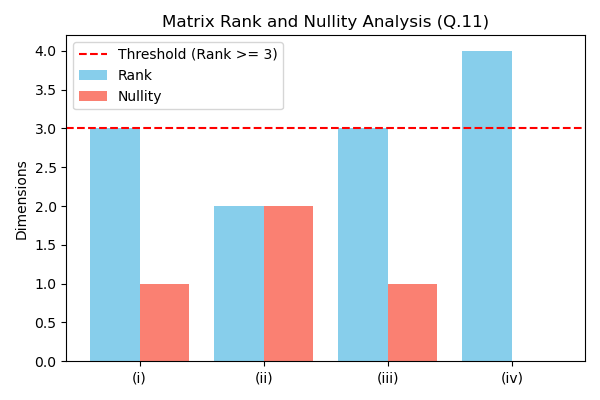
\includegraphics[width=0.90\linewidth]{figs/Matrix_Rank.png}
    \caption{Matrix Rank}
    \label{fig:EC2025-1-matrix-rank}
\end{figure}

\item
Consider the following series:
\begin{align}
\text{(i)}\ \sum_{n=1}^{\infty}\frac{1}{\sqrt{n}},\quad
\text{(ii)}\ \sum_{n=1}^{\infty}\frac{1}{n\brak{n+1}},\quad
\text{(iii)}\ \sum_{n=1}^{\infty}\frac{1}{n!}
\end{align}
Choose the correct option.
\hfill (EC~2025)
\begin{enumerate}
	\begin{multicols}{2}
    \item Only (ii) converges
    \item Only (ii) and (iii) converge
    \item Only (iii) converges
    \item All three converge
    \end{multicols}
\end{enumerate}
\solution
Series (i) is a $p$-series with $p=\frac{1}{2}$. From \eqref{eq:F-pseries},
\begin{align}
\sum_{n=1}^{\infty}\frac{1}{\sqrt{n}}&=\sum_{n=1}^{\infty}n^{-\frac{1}{2}}
\\
p=\frac{1}{2}&\le1
\\
\implies&\text{ (i) diverges}
\end{align}
Series (ii) telescopes. From \eqref{eq:F-telescope},
\begin{align}
\sum_{n=1}^{N}\frac{1}{n\brak{n+1}}&=1-\frac{1}{N+1}
\\
\lim_{N\to\infty}\brak{1-\frac{1}{N+1}}&=1
\end{align}
For series (iii), from \eqref{eq:F-ratio},
\begin{align}
\frac{a_{n+1}}{a_n}&=\frac{n!}{\brak{n+1}!}
\\
&=\frac{1}{n+1}
\\
\lim_{n\to\infty}\frac{1}{n+1}&=0<1
\end{align}
and from \eqref{eq:F-exp},
\begin{align}
\sum_{n=1}^{\infty}\frac{1}{n!}&=e-1
\end{align}
Hence, only (ii) and (iii) converge.

The following code verifies the solution through a plot
\begin{lstlisting}[frame=single, basicstyle=\rmfamily, escapeinside={(*@}{@*)}]
(*@\makebox[\dimexpr\linewidth-2\fboxsep-2\fboxrule\relax][c]{\texttt{\detokenize{codes/Series_Convergence.py}}}@*)
\end{lstlisting}
\begin{figure}[H]
    \centering
    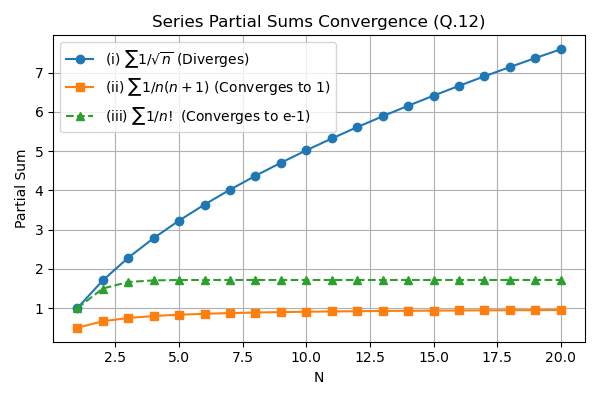
\includegraphics[width=0.90\linewidth]{figs/Series_Convergence.png}
    \caption{Series Convergence}
    \label{fig:EC2025-2-series-convergence}
\end{figure}

\item
A pot contains two red balls and two blue balls. Two balls are drawn from this pot randomly without replacement. What is the probability that the two balls drawn have different colours?
\hfill (EC~2025)
\begin{enumerate}
	\begin{multicols}{4}
    \item $\frac{2}{3}$
    \item $\frac{1}{3}$
    \item $\frac{1}{2}$
    \item $1$
    \end{multicols}
\end{enumerate}
\solution
Choosing two balls at random is the same as selecting each ball independently with probability $\frac{1}{2}$ and keeping the outcomes with exactly two balls selected. Let $B$ be the selection indicator of one ball, with
\begin{align}
p_B\sbrak{0}=p_B\sbrak{1}=\frac{1}{2}
\end{align}
The number $X$ of selected red balls is the sum of two independent indicators. From \eqref{eq:F-conv-pmf},
\begin{align}
p_X\sbrak{0}&=p_B\sbrak{0}p_B\sbrak{0}=\frac{1}{4}
\\
p_X\sbrak{1}&=p_B\sbrak{0}p_B\sbrak{1}+p_B\sbrak{1}p_B\sbrak{0}=\frac{1}{2}
\\
p_X\sbrak{2}&=p_B\sbrak{1}p_B\sbrak{1}=\frac{1}{4}
\end{align}
The number $Y$ of selected blue balls has $p_Y=p_X$. For $S=X+Y$, from \eqref{eq:F-conv-pmf},
\begin{align}
p_S\sbrak{2}&=p_X\sbrak{0}p_Y\sbrak{2}+p_X\sbrak{1}p_Y\sbrak{1}+p_X\sbrak{2}p_Y\sbrak{0}
\\
&=\frac{1}{16}+\frac{1}{4}+\frac{1}{16}
\\
&=\frac{3}{8}
\end{align}
The two balls have different colours when $X=1$ and $Y=1$. From \eqref{eq:F-indep},
\begin{align}
p_X\sbrak{1}p_Y\sbrak{1}&=\frac{1}{4}
\\
\pr{\text{different colours}}&=\frac{p_X\sbrak{1}p_Y\sbrak{1}}{p_S\sbrak{2}}
\\
&=\frac{\frac{1}{4}}{\frac{3}{8}}
\\
&=\frac{2}{3}
\end{align}

The following code verifies the solution through a plot
\begin{lstlisting}[frame=single, basicstyle=\rmfamily, escapeinside={(*@}{@*)}]
(*@\makebox[\dimexpr\linewidth-2\fboxsep-2\fboxrule\relax][c]{\texttt{\detokenize{codes/Two_balls.py}}}@*)
\end{lstlisting}
\begin{figure}[H]
    \centering
    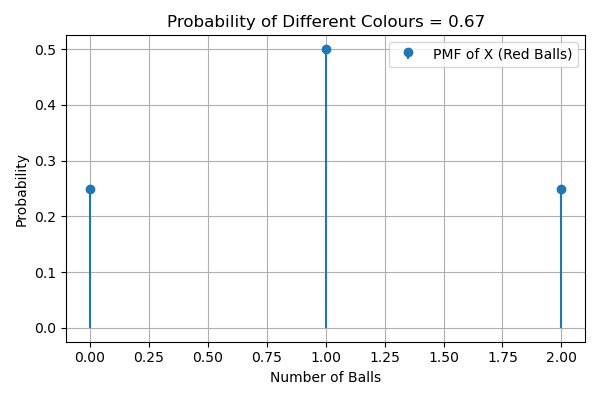
\includegraphics[width=0.90\linewidth]{figs/Two_balls.png}
    \caption{Two balls}
    \label{fig:EC2025-3-two-balls}
\end{figure}

\item
Consider a frequency-modulated (FM) signal
\begin{align}
f\brak{t}=A_c\cos\brak{2\pi f_ct+3\sin\brak{2\pi f_1t}+4\sin\brak{6\pi f_1t}}
\end{align}
where $A_c$ and $f_c$ are the amplitude and frequency (in Hz) of the carrier. The frequency $f_1$ is in Hz and $f_c>100f_1$. The peak frequency deviation of the FM signal in Hz is \underline{\hspace{1cm}}.
\hfill (EC~2025)
\begin{enumerate}
	\begin{multicols}{4}
    \item $15f_1$
    \item $12f_1$
    \item $4f_1$
    \item $2f_1$
    \end{multicols}
\end{enumerate}
\solution
The phase is
\begin{align}
\phi\brak{t}=2\pi f_ct+3\sin\brak{2\pi f_1t}+4\sin\brak{6\pi f_1t}
\end{align}
From \eqref{eq:F-fm},
\begin{align}
f_i\brak{t}&=\frac{1}{2\pi}\frac{d\phi}{dt}
\\
&=f_c+3f_1\cos\brak{2\pi f_1t}+12f_1\cos\brak{6\pi f_1t}
\\
\Delta f\brak{t}&=3f_1\cos\brak{2\pi f_1t}+12f_1\cos\brak{6\pi f_1t}
\end{align}
Both cosines equal $1$ at $t=0$, so
\begin{align}
\Delta f_{\text{peak}}&=3f_1+12f_1
\\
&=15f_1
\end{align}

The following code verifies the solution through a plot
\begin{lstlisting}[frame=single, basicstyle=\rmfamily, escapeinside={(*@}{@*)}]
(*@\makebox[\dimexpr\linewidth-2\fboxsep-2\fboxrule\relax][c]{\texttt{\detokenize{codes/FM_Dev.py}}}@*)
\end{lstlisting}
\begin{figure}[H]
    \centering
    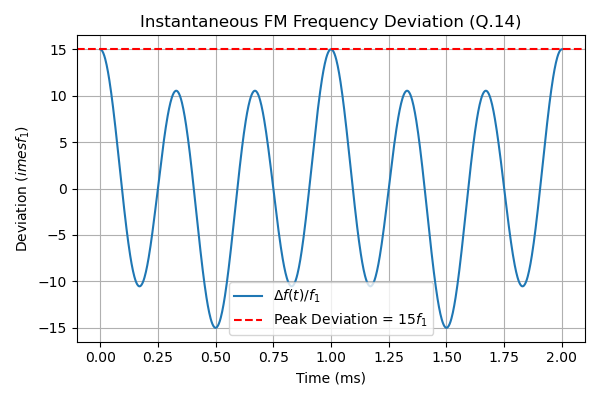
\includegraphics[width=0.90\linewidth]{figs/FM_Dev.png}
    \caption{FM Dev}
    \label{fig:EC2025-4-fm-dev}
\end{figure}

\item
Consider the discrete-time system in the given system diagram with input $x\sbrak{n}$ and output $y\sbrak{n}$. Here $h_1\sbrak{n}$ and $h_2\sbrak{n}$ are the impulse responses of LTI Subsystems 1 and 2, $\delta\sbrak{n}$ is the unit impulse, and $b>0$. Assuming $h_2\sbrak{n}\neq\delta\sbrak{n}$, the overall system (dashed box) is \underline{\hspace{1cm}}.
\hfill (EC~2025)
\begin{enumerate}
	\begin{multicols}{2}
    \item linear and time invariant
    \item linear and time variant
    \item nonlinear and time invariant
    \item nonlinear and time variant
    \end{multicols}
\end{enumerate}


\begin{figure}[H]
    \centering
    \begin{tikzpicture}[font=\footnotesize,>=Stealth,
        blk/.style={draw,minimum width=1.1cm,minimum height=0.7cm,inner sep=2pt},
        sm/.style={draw,circle,minimum size=0.5cm,inner sep=0pt}]
      % main chain
      \node (in)  at (0,0)   {$x[n]$};
      \node[blk] (h1) at (1.5,0) {$h_1[n]$};
      \node[sm]  (s1) at (2.9,0) {$+$};
      \node[blk] (h2) at (4.3,0) {$h_2[n]$};
      \node[sm]  (s2) at (5.7,0) {$+$};
      \node (out) at (6.8,0) {$y[n]$};
      \draw[->] (in.east)--(h1.west);
      \draw[->] (h1.east)--(s1.west);
      \draw[->] (s1.east)--(h2.west);
      \draw[->] (h2.east)--(s2.west);
      \draw[->] (s2.east)--(out.west);
      % impulse inputs
      \node (b1) at (2.9,-1.2) {$b\,\delta[n]$};
      \node (b2) at (5.7,-1.2) {$-b\,\delta[n]$};
      \draw[->] (b1.north)--(s1.south);
      \draw[->] (b2.north)--(s2.south);
      % labels and dashed box
      \node at (1.5,-0.65) {Subsystem 1};
      \node at (4.3,-0.65) {Subsystem 2};
      \draw[dashed] (0.75,0.7) rectangle (6.3,-1.65);
    \end{tikzpicture}
    \caption{Discrete-time system}
    \label{fig:q17}
\end{figure}

\solution
From the given system diagram and \eqref{eq:F-conv},
\begin{align}
y\sbrak{n}&=h_2\sbrak{n}*\brak{h_1\sbrak{n}*x\sbrak{n}+b\delta\sbrak{n}}-b\delta\sbrak{n}
\\
&=\brak{h_2*h_1*x}\sbrak{n}+b\brak{h_2\sbrak{n}-\delta\sbrak{n}}
\end{align}
For $x\sbrak{n}=0$,
\begin{align}
y\sbrak{n}&=b\brak{h_2\sbrak{n}-\delta\sbrak{n}}\neq0
\end{align}
which contradicts \eqref{eq:F-zero}, so the system is nonlinear. For a delayed input,
\begin{align}
T\cbrak{x\sbrak{n-k}}&=\brak{h_2*h_1*x}\sbrak{n-k}+b\brak{h_2\sbrak{n}-\delta\sbrak{n}}
\\
y\sbrak{n-k}&=\brak{h_2*h_1*x}\sbrak{n-k}+b\brak{h_2\sbrak{n-k}-\delta\sbrak{n-k}}
\end{align}
These differ, so \eqref{eq:F-ti} fails and the system is time variant.

The following code verifies the solution through a plot
\begin{lstlisting}[frame=single, basicstyle=\rmfamily, escapeinside={(*@}{@*)}]
(*@\makebox[\dimexpr\linewidth-2\fboxsep-2\fboxrule\relax][c]{\texttt{\detokenize{codes/LTI_System.py}}}@*)
\end{lstlisting}
\begin{figure}[H]
    \centering
    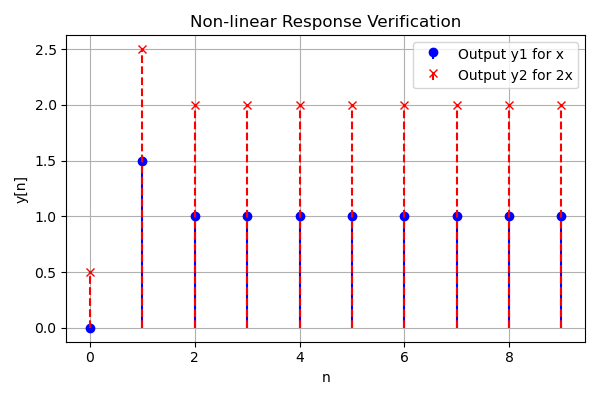
\includegraphics[width=0.90\linewidth]{figs/LTI_System.png}
    \caption{LTI System}
    \label{fig:EC2025-5-lti-system}
\end{figure}

\item
Consider a continuous-time, real-valued signal $f\brak{t}$ whose Fourier transform $F\brak{\omega}=\int_{-\infty}^{\infty}f\brak{t}e^{-\j\omega t}\,dt$ exists. Which one of the following statements is always TRUE?
\hfill (EC~2025)
\begin{enumerate}
	\begin{multicols}{2}
    \item $\abs{F\brak{\omega}}\le\int_{-\infty}^{\infty}\abs{f\brak{t}}\,dt$
    \item $\abs{F\brak{\omega}}>\int_{-\infty}^{\infty}\abs{f\brak{t}}\,dt$
    \item $\abs{F\brak{\omega}}\le\int_{-\infty}^{\infty}f\brak{t}\,dt$
    \item $\abs{F\brak{\omega}}\ge\int_{-\infty}^{\infty}f\brak{t}\,dt$
    \end{multicols}
\end{enumerate}
\solution
For $f\brak{t}=e^{-\abs{t}}$,
\begin{align}
\int_{-\infty}^{\infty}\abs{f\brak{t}}\,dt=\int_{-\infty}^{\infty}f\brak{t}\,dt=2
\end{align}
From \eqref{eq:F-ft-pair},
\begin{align}
\abs{F\brak{\omega}}&=\frac{2}{1+\omega^2}
\\
&\le2
\end{align}
with strict inequality for $\omega\neq0$, so (B) and (D) fail. For $g\brak{t}=-e^{-\abs{t}}$,
\begin{align}
\abs{G\brak{0}}&=2
\\
\int_{-\infty}^{\infty}g\brak{t}\,dt&=-2
\end{align}
so (C) fails. From \eqref{eq:F-ft-bound},
\begin{align}
\abs{F\brak{\omega}}&\le\int_{-\infty}^{\infty}\abs{f\brak{t}}\abs{e^{-\j\omega t}}\,dt
\\
&=\int_{-\infty}^{\infty}\abs{f\brak{t}}\,dt
\end{align}
for every signal, so (A) is true.

The following code verifies the solution through a plot
\begin{lstlisting}[frame=single, basicstyle=\rmfamily, escapeinside={(*@}{@*)}]
(*@\makebox[\dimexpr\linewidth-2\fboxsep-2\fboxrule\relax][c]{\texttt{\detokenize{codes/Fourier_Bound.py}}}@*)
\end{lstlisting}
\begin{figure}[H]
    \centering
    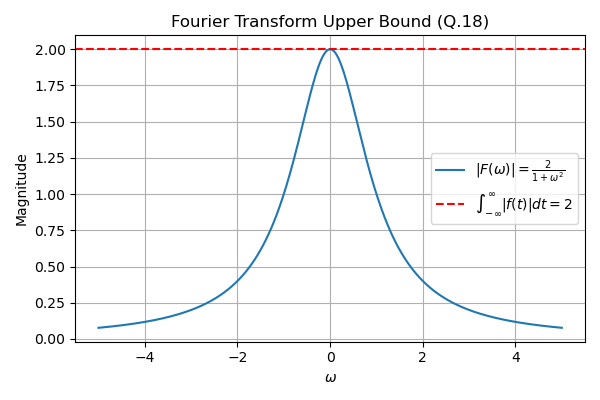
\includegraphics[width=0.90\linewidth]{figs/Fourier_Bound.png}
    \caption{Fourier Bound}
    \label{fig:EC2025-6-fourier-bound}
\end{figure}

\item
Let $i_C$, $i_L$ and $i_R$ be the currents through the capacitor, inductor and resistor in the circuit of the given parallel RLC circuit. The AC admittances are given in Siemens (S). Which one of the following is TRUE?
\hfill (EC~2025)
\begin{enumerate}
	\begin{multicols}{2}
    \item $i_C=0.25\angle180^\circ$ A, $i_L=0.1\angle0^\circ$ A, $i_R=0.2\angle90^\circ$ A
    \item $i_C=4\angle180^\circ$ A, $i_L=10\angle0^\circ$ A, $i_R=5\angle90^\circ$ A
    \item $i_C=0.25\angle270^\circ$ A, $i_L=0.1\angle90^\circ$ A, $i_R=0.2\angle90^\circ$ A
    \item $i_C=4\angle90^\circ$ A, $i_L=10\angle270^\circ$ A, $i_R=5\angle0^\circ$ A
    \end{multicols}
\end{enumerate}


\begin{figure}[H]
    \centering
    \begin{tikzpicture}[font=\footnotesize,>=Stealth]
      % top and bottom rails
      \draw (0,3)--(5.2,3);
      \draw (0,0)--(5.2,0);
      % voltage source
      \draw (0,3)--(0,2);
      \draw (0,1)--(0,0);
      \draw (0,1.5) circle (0.5);
      \draw (-0.3,1.5) sin (-0.15,1.7) cos (0,1.5) sin (0.15,1.3) cos (0.3,1.5);
      \node at (0.33,2.3) {$+$};
      \node at (0.33,0.7) {$-$};
      \node[left] at (-0.6,1.5) {$1\angle 90^\circ$ V};
      % junction dots
      \fill (1.8,3) circle (1.2pt);
      \fill (3.5,3) circle (1.2pt);
      \fill (1.8,0) circle (1.2pt);
      \fill (3.5,0) circle (1.2pt);
      % capacitor branch
      \draw (1.8,3)--(1.8,1.7);
      \draw (1.5,1.7)--(2.1,1.7);
      \draw (1.5,1.3)--(2.1,1.3);
      \draw (1.8,1.3)--(1.8,0);
      \node[right] at (2.1,1.5) {$j0.25$ S};
      \draw[->] (1.3,2.7)--(1.3,2.1);
      \node[left] at (1.3,2.4) {$i_C$};
      % inductor branch
      \draw (3.5,3)--(3.5,2.4);
      \draw[decorate,decoration={coil,aspect=0.5,segment length=3.5pt,amplitude=3.5pt}] (3.5,2.4)--(3.5,0.6);
      \draw (3.5,0.6)--(3.5,0);
      \node[right] at (3.75,1.5) {$-j0.1$ S};
      \draw[->] (3.1,2.7)--(3.1,2.1);
      \node[left] at (3.1,2.4) {$i_L$};
      % resistor branch
      \draw (5.2,3)--(5.2,2.4);
      \draw[decorate,decoration={zigzag,segment length=4pt,amplitude=3pt}] (5.2,2.4)--(5.2,0.6);
      \draw (5.2,0.6)--(5.2,0);
      \node[right] at (5.45,1.5) {$0.2$ S};
      \draw[->] (4.8,2.7)--(4.8,2.1);
      \node[left] at (4.8,2.4) {$i_R$};
    \end{tikzpicture}
    \caption{Parallel $R$, $L$, $C$ branches}
    \label{fig:q20}
\end{figure}

\solution
All three branches are connected in parallel, so each branch has the source voltage
$\underline{V}=1\angle90^\circ$ V across it. Using $\underline{I}=\underline{Y}\,\underline{V}$:
\begin{align}
\underline{I}_C&=(\j0.25)(1\angle90^\circ)
=0.25\angle180^\circ\text{ A},\\
\underline{I}_L&=(-\j0.1)(1\angle90^\circ)
=0.1\angle0^\circ\text{ A},\\
\underline{I}_R&=(0.2)(1\angle90^\circ)
=0.2\angle90^\circ\text{ A}.
\end{align}
Therefore, the correct choice is **Option (A)**. The original numerical solution is correct.

The following code verifies the solution through a plot
\begin{lstlisting}[frame=single, basicstyle=\rmfamily, escapeinside={(*@}{@*)}]
(*@\makebox[\dimexpr\linewidth-2\fboxsep-2\fboxrule\relax][c]{\texttt{\detokenize{codes/AC_Admittance.py}}}@*)
\end{lstlisting}
\begin{figure}[H]
    \centering
    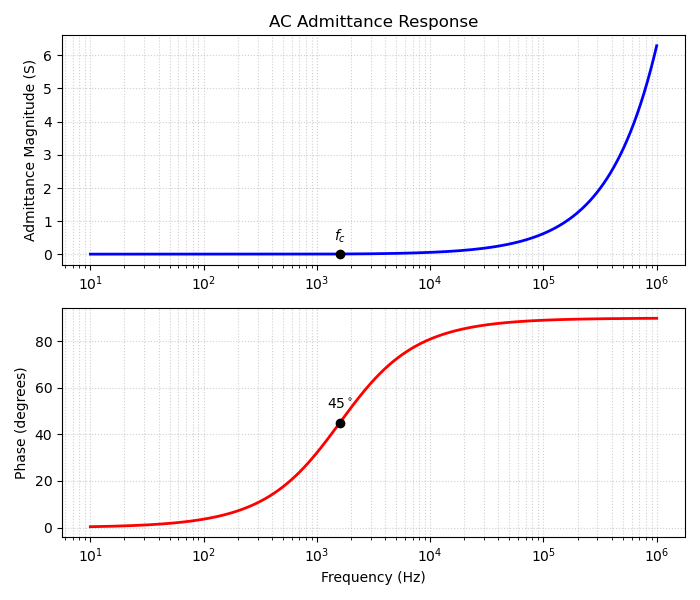
\includegraphics[width=0.90\linewidth]{figs/AC_Admittance.png}
    \caption{AC Admittance}
    \label{fig:EC2025-7-ac-admittance}
\end{figure}

\item
A 3-input majority logic gate has inputs $X$, $Y$, $Z$. The output $F$ is logic `1' if two or more inputs are logic `1', and logic `0' if two or more inputs are logic `0'. Which one of the following is a Boolean expression of $F$?
\hfill (EC~2025)
\begin{enumerate}
	\begin{multicols}{4}
    \item $XY+YZ+ZX$
    \item $X\oplus Y\oplus Z$
    \item $X+Y+Z$
    \item $XYZ$
    \end{multicols}
\end{enumerate}
\solution
$F=1$ for the inputs $011,101,110,111$. Pairing each of the first three minterms with $XYZ$,
\begin{align}
F&=\overline{X}YZ+X\overline{Y}Z+XY\overline{Z}+XYZ
\\
&=\brak{\overline{X}YZ+XYZ}+\brak{X\overline{Y}Z+XYZ}+\brak{XY\overline{Z}+XYZ}
\\
&=YZ+XZ+XY
\end{align}
which is \eqref{eq:F-maj}. The truth table is
\begin{center}
\begin{tabular}{|c|c|c|c|c|c|c|c|}
\hline
$X$&$Y$&$Z$&$F$&$XY+YZ+ZX$&$X\oplus Y\oplus Z$&$X+Y+Z$&$XYZ$\\
\hline
0&0&0&0&0&0&0&0\\
0&0&1&0&0&1&1&0\\
0&1&0&0&0&1&1&0\\
0&1&1&1&1&0&1&0\\
1&0&0&0&0&1&1&0\\
1&0&1&1&1&0&1&0\\
1&1&0&1&1&0&1&0\\
1&1&1&1&1&1&1&1\\
\hline
\end{tabular}
\end{center}

The following code verifies the solution.
\begin{lstlisting}[frame=single, basicstyle=\rmfamily, escapeinside={(*@}{@*)}]
(*@\makebox[\dimexpr\linewidth-2\fboxsep-2\fboxrule\relax][c]{\texttt{\detokenize{codes/Majority_Gate.c}}}@*)
\end{lstlisting}

\item
A full adder and an XOR gate are used to design a digital circuit with inputs $X$, $Y$, $Z$ and output $F$, as in the given logic circuit. The input $Z$ is connected to the carry-in of the full adder. If $Z$ is set to logic `1', the circuit functions as \underline{\hspace{1cm}} with $X$ and $Y$ as inputs.
\hfill (EC~2025)
\begin{enumerate}
	\begin{multicols}{2}
    \item an adder
    \item a subtractor
    \item a multiplier
    \item a binary to Gray code converter
    \end{multicols}
\end{enumerate}


\begin{figure}[H]
    \centering
    \begin{tikzpicture}[font=\footnotesize,>=Stealth]
      % full adder
      \draw (-1.2,0)--(1.2,0)--(0.8,-1)--(-0.8,-1)--cycle;
      \node[align=center] at (0,-0.5) {full\\adder};
      % inputs
      \node at (-0.8,2.55) {$X$};
      \node at (0.2,2.55) {$Y$};
      \node at (0.6,2.55) {$Z$};
      \draw[->] (-0.8,2.35)--(-0.8,0);
      \draw (0.2,2.35)--(0.2,1.26);
      \draw (0.6,2.35)--(0.6,1.26);
      % XOR gate (pointing down)
      \begin{scope}[shift={(0.4,1.0)}]
        \draw (-0.4,0.35) .. controls (-0.2,0.2) and (0.2,0.2) .. (0.4,0.35);
        \draw (-0.4,0.35) .. controls (-0.4,-0.05) and (-0.15,-0.3) .. (0,-0.4);
        \draw (0.4,0.35) .. controls (0.4,-0.05) and (0.15,-0.3) .. (0,-0.4);
        \draw (-0.4,0.47) .. controls (-0.2,0.32) and (0.2,0.32) .. (0.4,0.47);
      \end{scope}
      \draw[->] (0.4,0.6)--(0.4,0);
      % Z to carry-in
      \fill (0.6,1.8) circle (1.2pt);
      \draw[->] (0.6,1.8)--(1.7,1.8)--(1.7,-0.5)--(1.0,-0.5);
      % output
      \draw[->] (0,-1)--(0,-1.8);
      \draw (-0.08,-1.48)--(0.08,-1.32);
      \node[right] at (0.05,-1.4) {\scriptsize 2};
      \node at (0,-2.05) {$F$};
    \end{tikzpicture}
    \caption{Full adder with an XOR gate}
    \label{fig:q24}
\end{figure}

\solution
From the given logic circuit, the XOR gate forms $Y\oplus Z$ and $Z$ is the carry-in. For $Z=1$, from \eqref{eq:F-xor},
\begin{align}
Y\oplus1&=\overline{Y}
\end{align}
From \eqref{eq:F-twos},
\begin{align}
F&=X+\overline{Y}+1
\\
&\equiv X-Y\pmod{2^n}
\end{align}
so the circuit is a subtractor.

The following code verifies the solution through a plot
\begin{lstlisting}[frame=single, basicstyle=\rmfamily, escapeinside={(*@}{@*)}]
(*@\makebox[\dimexpr\linewidth-2\fboxsep-2\fboxrule\relax][c]{\texttt{\detokenize{codes/Adder_Subtractor.py}}}@*)
\end{lstlisting}
\begin{figure}[H]
    \centering
    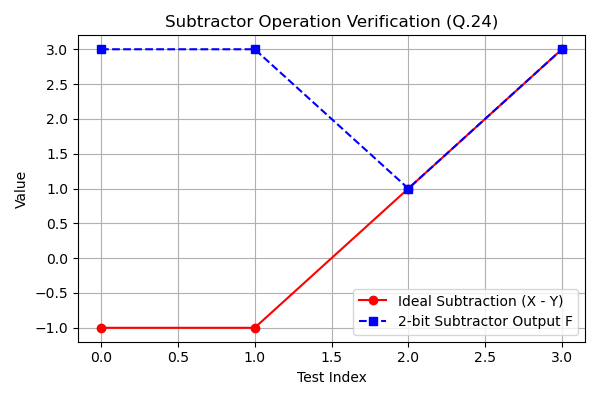
\includegraphics[width=0.90\linewidth]{figs/Adder_Subtractor.png}
    \caption{Adder Subtractor}
    \label{fig:EC2025-9-adder-subtractor}
\end{figure}

\item
Consider $f:\mathbb{R}\to\mathbb{R}$ defined by $f\brak{x}=2x^3-3x^2-12x+1$. Which of the following statements is/are correct?
\hfill (EC~2025)
\begin{enumerate}
	\begin{multicols}{2}
    \item $f$ has no global maximizer
    \item $f$ has no global minimizer
    \item $x=-1$ is a local minimizer of $f$
    \item $x=2$ is a local maximizer of $f$
    \end{multicols}
\end{enumerate}
\solution
\begin{align}
f^{\prime}\brak{x}&=6x^2-6x-12
\\
&=6\brak{x+1}\brak{x-2}
\\
f^{\prime\prime}\brak{x}&=12x-6
\end{align}
From \eqref{eq:F-second},
\begin{align}
f^{\prime\prime}\brak{-1}&=-18<0
\\
\implies x&=-1\text{ is a local maximum}
\\
f^{\prime\prime}\brak{2}&=18>0
\\
\implies x&=2\text{ is a local minimum}
\end{align}
So (C) and (D) are false. Also,
\begin{align}
\lim_{x\to\infty}f\brak{x}&=+\infty
\\
\lim_{x\to-\infty}f\brak{x}&=-\infty
\end{align}
so $f$ has neither a global maximizer nor a global minimizer.

The following code verifies the solution through a plot
\begin{lstlisting}[frame=single, basicstyle=\rmfamily, escapeinside={(*@}{@*)}]
(*@\makebox[\dimexpr\linewidth-2\fboxsep-2\fboxrule\relax][c]{\texttt{\detokenize{codes/Cubic_Extrema.py}}}@*)
\end{lstlisting}
\begin{figure}[H]
    \centering
    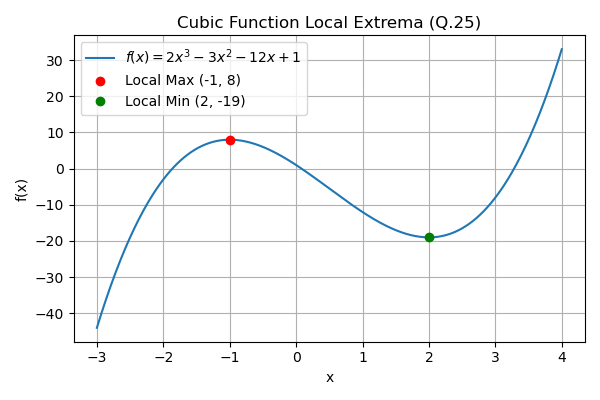
\includegraphics[width=0.90\linewidth]{figs/Cubic_Extrema.png}
    \caption{Cubic Extrema}
    \label{fig:EC2025-10-cubic-extrema}
\end{figure}

\item
Consider the unity-negative-feedback system in the given unity-negative-feedback system, where the gain $K\ge0$. The root locus of this system is shown in the given root-locus plot. For what value(s) of $K$ will the system in the given unity-negative-feedback system have a pole at $-1+\j1$?
\hfill (EC~2025)
\begin{enumerate}
	\begin{multicols}{2}
    \item $K=5$
    \item $K=\frac{1}{5}$
    \item For no positive value of $K$
    \item For all positive values of $K$
    \end{multicols}
\end{enumerate}


\begin{figure}[H]
    \centering
    \begin{tikzpicture}[font=\footnotesize,>=Stealth,
        blk/.style={draw,minimum width=1cm,minimum height=0.7cm,inner sep=3pt}]
      \node (R) at (-1.8,0) {$R(s)$};
      \node[draw,circle,minimum size=0.6cm,inner sep=0pt] (sum) at (0,0) {};
      \draw (sum.north west)--(sum.south east);
      \draw (sum.north east)--(sum.south west);
      \node[blk] (K) at (1.7,0) {$K$};
      \node[blk] (G) at (3.4,0) {$G(s)$};
      \node (Y) at (5.4,0) {$Y(s)$};
      \draw[->] (R.east)--(sum.west);
      \draw[->] (sum.east)--(K.west);
      \draw[->] (K.east)--(G.west);
      \draw[->] (G.east)--(Y.west);
      \fill (4.5,0) circle (1.2pt);
      \draw[->] (4.5,0)--(4.5,-1.2)--(0,-1.2)--(sum.south);
      \node at ($(sum.west)+(-0.25,0.22)$) {$+$};
      \node at ($(sum.south)+(0.25,-0.25)$) {$-$};
    \end{tikzpicture}
    \caption{Unity-negative-feedback system}
    \label{fig:q26a}
\end{figure}

\begin{figure}[H]
    \centering
    \begin{tikzpicture}[x=1.6cm,y=1.6cm,font=\footnotesize,>=Stealth]
      % dashed grid lines
      \foreach \x in {-4,-3,-2,-1} {\draw[dashed,gray] (\x,-1.2)--(\x,1);}
      \draw[dashed,gray] (-4.6,1)--(-1,1);
      \draw[dotted,gray] (-4.6,0)--(-4,0);
      % axes
      \draw[->] (-4.6,-1.2)--(-0.6,-1.2);
      \draw[->] (-4.6,-1.2)--(-4.6,1.4);
      \foreach \x in {-4,-3,-2,-1} {
        \draw (\x,-1.2)--(\x,-1.27);
        \node[below] at (\x,-1.27) {$\x$};
      }
      \foreach \y in {-1,0,1} {\draw (-4.6,\y)--(-4.53,\y);}
      \node[left] at (-4.6,1) {$j1$};
      \node[left] at (-4.6,0) {$0$};
      \node[left] at (-4.6,-1) {$-j1$};
      \node[rotate=90] at (-5.35,0) {Imaginary axis};
      \node at (-2.5,-1.75) {Real axis};
      % root locus branches
      \draw[thick] (-4,0)--(-3,0);
      \draw[thick] (-2,0)--(-1,0);
      \draw[thick] (-2.5,0) circle (0.866);
      % direction arrows
      \draw[thick,-{Stealth[length=2mm]}] (-3.5,0)--(-3.8,0);
      \draw[thick,-{Stealth[length=2mm]}] (-3.3,0)--(-3.12,0);
      \draw[thick,-{Stealth[length=2mm]}] (-1.9,0)--(-1.72,0);
      \draw[thick,-{Stealth[length=2mm]}] (-1.1,0)--(-1.28,0);
      \draw[thick,-{Stealth[length=2mm]}] (-2.3,0.866)--(-2.5,0.866);
      \draw[thick,-{Stealth[length=2mm]}] (-2.3,-0.866)--(-2.5,-0.866);
      % open-loop zeros (o) and poles (x)
      \foreach \x in {-4,-3} {\draw[thick,fill=white] (\x,0) circle (2.5pt);}
      \foreach \x in {-2,-1} {
        \draw[thick] (\x,0)+(-2.5pt,-2.5pt)--+(2.5pt,2.5pt);
        \draw[thick] (\x,0)+(-2.5pt,2.5pt)--+(2.5pt,-2.5pt);
      }
      % legend
      \draw (-4.5,-2.0) rectangle (-2.7,-2.55);
      \draw[thick,fill=white] (-4.35,-2.14) circle (2.5pt);
      \node[anchor=west,font=\scriptsize] at (-4.25,-2.14) {Open loop zeros};
      \draw[thick] (-4.35,-2.4)+(-2.5pt,-2.5pt)--+(2.5pt,2.5pt);
      \draw[thick] (-4.35,-2.4)+(-2.5pt,2.5pt)--+(2.5pt,-2.5pt);
      \node[anchor=west,font=\scriptsize] at (-4.25,-2.4) {Open loop poles};
    \end{tikzpicture}
    \caption{Root locus of the system}
    \label{fig:q26b}
\end{figure}

\solution
From the given root-locus plot,
\begin{align}
G\brak{s}=\frac{\brak{s+3}\brak{s+4}}{\brak{s+1}\brak{s+2}}
\end{align}
From \eqref{eq:F-rootlocus}, at $s_0=-1+\j$,
\begin{align}
G\brak{s_0}&=\frac{\brak{2+\j}\brak{3+\j}}{\j\brak{1+\j}}
\\
&=\frac{5+5\j}{-1+\j}
\\
&=-5\j
\end{align}
which is not real, so $s_0$ is not on the root locus for any $K$.

The following code verifies the solution through a plot
\begin{lstlisting}[frame=single, basicstyle=\rmfamily, escapeinside={(*@}{@*)}]
(*@\makebox[\dimexpr\linewidth-2\fboxsep-2\fboxrule\relax][c]{\texttt{\detokenize{codes/Root_Locus.py}}}@*)
\end{lstlisting}
\begin{figure}[H]
    \centering
    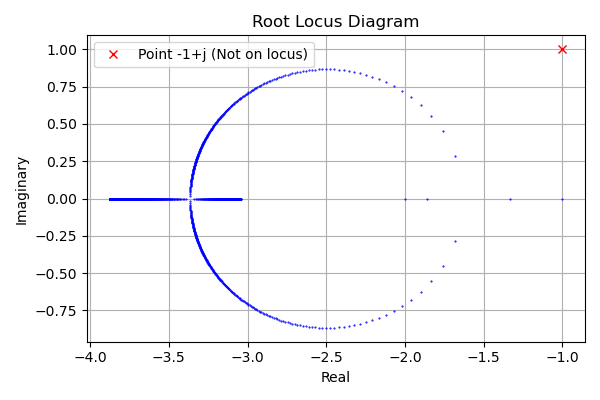
\includegraphics[width=0.90\linewidth]{figs/Root_Locus.png}
    \caption{Root Locus}
    \label{fig:EC2025-11-root-locus}
\end{figure}

\item
Let $x\sbrak{n}$ be a discrete-time signal whose $z$-transform is $X\brak{z}$. Which of the following statements is/are TRUE?
\hfill (EC~2025)
\begin{enumerate}
    \item The discrete-time Fourier transform (DTFT) of $x\sbrak{n}$ always exists
    \item The region of convergence (RoC) of $X\brak{z}$ contains neither poles nor zeros
    \item The DTFT exists if the RoC contains the unit circle
    \item If $x\sbrak{n}=\alpha\delta\sbrak{n}$, where $\delta\sbrak{n}$ is the unit impulse and $\alpha$ is a scalar, then the RoC is the entire $z$-plane
\end{enumerate}
\solution
For $x\sbrak{n}=2^nu\sbrak{n}$ the RoC is $\abs{z}>2$, which excludes the unit circle, so (A) is false. For
\begin{align}
x\sbrak{n}&=\delta\sbrak{n}-0.5\delta\sbrak{n-1}
\\
X\brak{z}&=1-0.5z^{-1}
\\
&=\frac{z-0.5}{z}
\end{align}
the zero $z=0.5$ lies in the RoC, so (B) is false. From \eqref{eq:F-ztrans}, (C) is true. For $x\sbrak{n}=\alpha\delta\sbrak{n}$,
\begin{align}
X\brak{z}&=\alpha\sum_{n}\delta\sbrak{n}z^{-n}
\\
&=\alpha
\end{align}
which is finite for every $z$, so (D) is true.

The following code verifies the solution through a plot
\begin{lstlisting}[frame=single, basicstyle=\rmfamily, escapeinside={(*@}{@*)}]
(*@\makebox[\dimexpr\linewidth-2\fboxsep-2\fboxrule\relax][c]{\texttt{\detokenize{codes/Z_Transform.py}}}@*)
\end{lstlisting}
\begin{figure}[H]
    \centering
    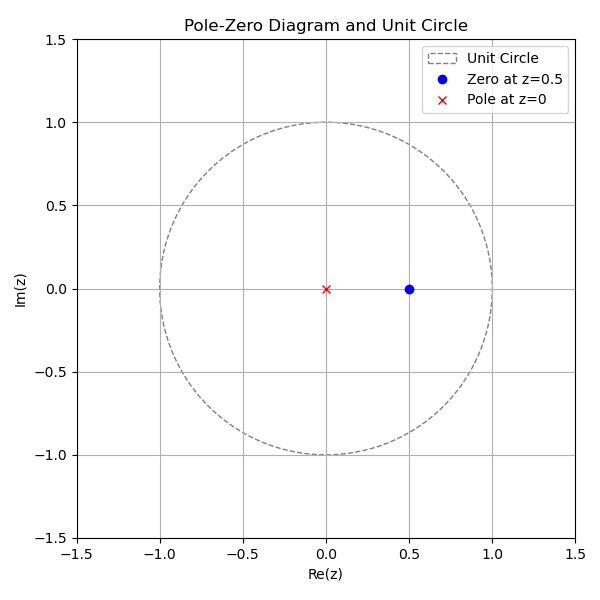
\includegraphics[width=0.90\linewidth]{figs/Z_Transform.png}
    \caption{Z Transform}
    \label{fig:EC2025-12-z-transform}
\end{figure}

\item
Consider a message signal $m\brak{t}$ bandlimited to $\sbrak{-W,W}$ ($W$ in Hz) and two schemes:
\begin{align}
\text{DSB-SC: }f_{DSB}\brak{t}&=A_cm\brak{t}\cos\brak{2\pi f_ct}
\\
\text{AM: }f_{AM}\brak{t}&=A_c\brak{1+\mu m\brak{t}}\cos\brak{2\pi f_ct}
\end{align}
Here $A_c$, $f_c$ are the carrier amplitude and frequency, and $\mu$ is the modulation index. Consider the statements:
\\
(i) An envelope detector can be used for demodulation in the DSB-SC scheme if $m\brak{t}>0$ for all $t$.
\\
(ii) An envelope detector can be used for demodulation in the AM scheme only if $m\brak{t}>0$ for all $t$.
\\
Which of the following options is/are correct?
\hfill (EC~2025)
\begin{enumerate}
	\begin{multicols}{4}
    \item (i) is TRUE
    \item (i) is FALSE
    \item (ii) is TRUE
    \item (ii) is FALSE
    \end{multicols}
\end{enumerate}
\solution
From \eqref{eq:F-envelope}, for DSB-SC with $m\brak{t}>0$,
\begin{align}
A_c\abs{m\brak{t}}&=A_cm\brak{t}
\end{align}
so (i) is true. For AM, recovery needs only $1+\mu m\brak{t}\ge0$. For $m\brak{t}=\cos\brak{2\pi Wt}$ and $\mu=\frac{1}{2}$,
\begin{align}
1+\mu m\brak{t}&\ge\frac{1}{2}
\\
&>0
\end{align}
although $m\brak{t}$ is negative half the time, so (ii) is false.

The following code verifies the solution through a plot
\begin{lstlisting}[frame=single, basicstyle=\rmfamily, escapeinside={(*@}{@*)}]
(*@\makebox[\dimexpr\linewidth-2\fboxsep-2\fboxrule\relax][c]{\texttt{\detokenize{codes/Envelope_Detector.py}}}@*)
\end{lstlisting}
\begin{figure}[H]
    \centering
    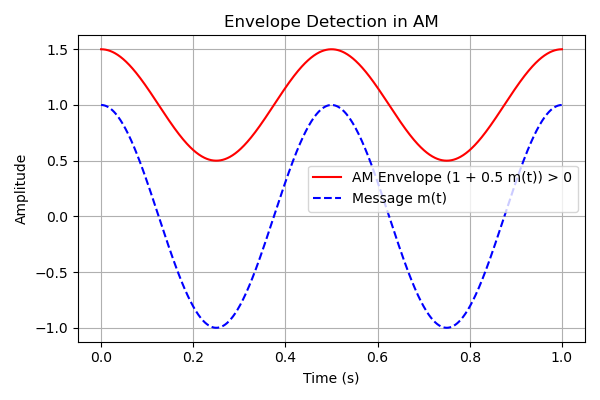
\includegraphics[width=0.90\linewidth]{figs/Envelope_Detector.png}
    \caption{Envelope Detector}
    \label{fig:EC2025-13-envelope-detector}
\end{figure}

\item
The function $y\brak{t}$ satisfies $t^2y^{\prime\prime}\brak{t}-2ty^{\prime}\brak{t}+2y\brak{t}=0$, where $y^{\prime}$ and $y^{\prime\prime}$ are the first and second derivatives. Given $y^{\prime}\brak{0}=1$ and $y^{\prime}\brak{1}=-1$, the maximum value of $y\brak{t}$ over $\sbrak{0,1}$ is \underline{\hspace{1cm}} (rounded off to two decimal places).
\hfill (EC~2025)
\\
\solution
From \eqref{eq:F-euler-cauchy},
\begin{align}
m\brak{m-1}-2m+2&=0
\\
\implies\brak{m-1}\brak{m-2}&=0
\\
\implies y&=C_1t+C_2t^2
\\
y^{\prime}&=C_1+2C_2t
\end{align}
Substituting $y^{\prime}\brak{0}=1$ and $y^{\prime}\brak{1}=-1$,
\begin{align}
C_1&=1
\\
1+2C_2&=-1
\\
\implies C_2&=-1
\\
y&=t-t^2
\end{align}
From \eqref{eq:F-second},
\begin{align}
y^{\prime}&=1-2t=0
\\
\implies t&=\frac{1}{2}
\\
y_{\max}&=\frac{1}{2}-\frac{1}{4}
\\
&=0.25
\end{align}

The following code verifies the solution.
\begin{lstlisting}[frame=single, basicstyle=\rmfamily, escapeinside={(*@}{@*)}]
(*@\makebox[\dimexpr\linewidth-2\fboxsep-2\fboxrule\relax][c]{\texttt{\detokenize{codes/Euler_Cauchy.c}}}@*)
\end{lstlisting}

\item
The generator matrix of a $\brak{6,3}$ binary linear block code is
\begin{align}
\vec{G}=\myvec{1&0&0&1&0&1\\0&1&0&0&1&1\\0&0&1&1&1&0}
\end{align}
The minimum Hamming distance $d_{\min}$ between codewords equals \underline{\hspace{1cm}} (answer in integer).
\hfill (EC~2025)
\\
\solution
The codewords are $\vec{c}=\vec{u}\vec{G}$ (mod 2):
\begin{center}
\begin{tabular}{|c|c|c|}
\hline
$\vec{u}$&$\vec{c}$&$w\brak{\vec{c}}$\\
\hline
001&001110&3\\
010&010011&3\\
011&011101&4\\
100&100101&3\\
101&101011&4\\
110&110110&4\\
111&111000&3\\
\hline
\end{tabular}
\end{center}
From \eqref{eq:F-dmin},
\begin{align}
d_{\min}&=\min_{\vec{c}\neq\vec{0}}w\brak{\vec{c}}
\\
&=3
\end{align}

The following code verifies the solution through a plot
\begin{lstlisting}[frame=single, basicstyle=\rmfamily, escapeinside={(*@}{@*)}]
(*@\makebox[\dimexpr\linewidth-2\fboxsep-2\fboxrule\relax][c]{\texttt{\detokenize{codes/Linear_Block_Code.py}}}@*)
\end{lstlisting}
\begin{figure}[H]
    \centering
    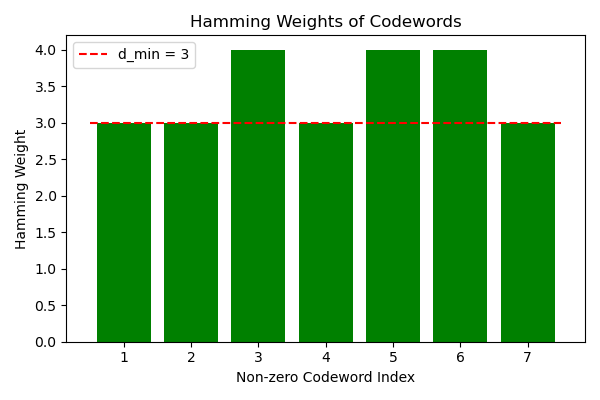
\includegraphics[width=0.90\linewidth]{figs/Linear_Block_Code.png}
    \caption{Linear Block Code}
    \label{fig:EC2025-15-linear-block-code}
\end{figure}

\item
All components in the bandpass filter of the given bandpass filter are ideal. The lower $-3$ dB frequency is 1 MHz. The upper $-3$ dB frequency (in MHz, rounded off to the nearest integer) is \underline{\hspace{1cm}}.
\hfill (EC~2025)


\begin{figure}[H]
    \centering
    \begin{tikzpicture}[font=\footnotesize,>=Stealth,
        zz/.style={decorate,decoration={zigzag,segment length=4pt,amplitude=3pt}}]
      % op-amp
      \draw (3,1)--(3,-1)--(5,0)--cycle;
      \node at (3.25,0.5) {$-$};
      \node at (3.25,-0.5) {$+$};
      % input branch: vs - R - 10C - inverting input
      \draw (0,0.5)--(0.4,0.5);
      \draw[zz] (0.4,0.5)--(1.3,0.5);
      \draw (1.3,0.5)--(1.65,0.5);
      \draw (1.65,0.3)--(1.65,0.7);
      \draw (1.85,0.3)--(1.85,0.7);
      \draw (1.85,0.5)--(3,0.5);
      \draw[fill=white] (0,0.5) circle (1.5pt);
      \node[left] at (-0.1,0.5) {$v_s$};
      \node at (0.85,0.9) {$R$};
      \node at (1.75,0.95) {$10C$};
      % feedback: 2R
      \fill (2.5,0.5) circle (1.2pt);
      \draw (2.5,0.5)--(2.5,2.4)--(3.2,2.4);
      \draw[zz] (3.2,2.4)--(4.5,2.4);
      \draw (4.5,2.4)--(5.2,2.4)--(5.2,0);
      \node at (3.85,2.8) {$2R$};
      % feedback: 0.1C
      \fill (2.5,1.5) circle (1.2pt);
      \fill (5.2,1.5) circle (1.2pt);
      \draw (2.5,1.5)--(3.75,1.5);
      \draw (3.75,1.3)--(3.75,1.7);
      \draw (3.95,1.3)--(3.95,1.7);
      \draw (3.95,1.5)--(5.2,1.5);
      \node at (3.85,1.95) {$0.1C$};
      % output
      \draw (5,0)--(5.7,0);
      \fill (5.2,0) circle (1.2pt);
      \draw[fill=white] (5.7,0) circle (1.5pt);
      \node[right] at (5.8,0) {$v_o$};
      % grounded non-inverting input
      \draw (3,-0.5)--(2.5,-0.5)--(2.5,-1.0);
      \draw (2.3,-1.0)--(2.7,-1.0);
      \draw (2.38,-1.1)--(2.62,-1.1);
      \draw (2.46,-1.2)--(2.54,-1.2);
    \end{tikzpicture}
    \caption{Active bandpass filter}
    \label{fig:q34}
\end{figure}

\solution
From the given bandpass filter,
\begin{align}
Z_i&=R+\frac{1}{s10C}
\\
&=\frac{1+10sRC}{10sC}
\\
Z_f&=\frac{2R}{1+0.2sRC}
\end{align}
From \eqref{eq:F-inv},
\begin{align}
H\brak{s}&=-\frac{Z_f}{Z_i}
\\
&=-\frac{20sRC}{\brak{1+10sRC}\brak{1+0.2sRC}}
\end{align}
From \eqref{eq:F-corner},
\begin{align}
\omega_L&=\frac{1}{10RC}
\\
\omega_H&=\frac{1}{0.2RC}
\\
\frac{f_H}{f_L}&=\frac{10RC}{0.2RC}
\\
&=50
\\
f_H&=50\times1\text{ MHz}
\\
&=50\text{ MHz}
\end{align}

The following code verifies the solution through a plot
\begin{lstlisting}[frame=single, basicstyle=\rmfamily, escapeinside={(*@}{@*)}]
(*@\makebox[\dimexpr\linewidth-2\fboxsep-2\fboxrule\relax][c]{\texttt{\detokenize{codes/Bandpass_Filter.py}}}@*)
\end{lstlisting}
\begin{figure}[H]
    \centering
    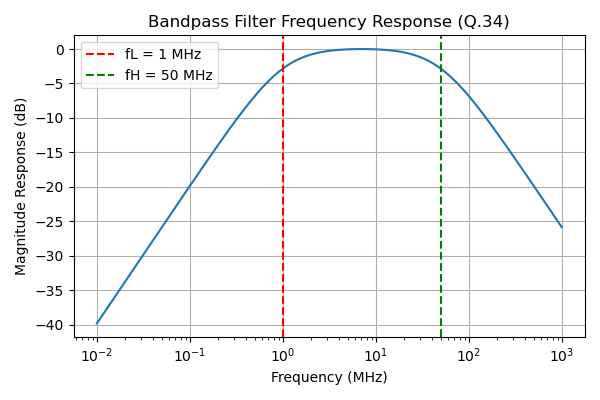
\includegraphics[width=0.90\linewidth]{figs/Bandpass_Filter.png}
    \caption{Bandpass Filter}
    \label{fig:EC2025-16-bandpass-filter}
\end{figure}

\item
Let $G\brak{s}=\frac{1}{10s^2}$ be the transfer function of a second-order system. A controller $M\brak{s}$ is connected to $G\brak{s}$ in the configuration of the given feedback configuration. Consider:
\\
(i) There exists no controller $M\brak{s}=\frac{K_I}{s}$, with $K_I$ a positive real number, such that the closed-loop system is stable.
\\
(ii) There exists at least one controller $M\brak{s}=K_P+sK_D$, with $K_P,K_D$ positive real numbers, such that the closed-loop system is stable.
\\
Which one of the following options is correct?
\hfill (EC~2025)
\begin{enumerate}
	\begin{multicols}{2}
    \item (i) is TRUE and (ii) is FALSE
    \item (i) is FALSE and (ii) is TRUE
    \item Both (i) and (ii) are FALSE
    \item Both (i) and (ii) are TRUE
    \end{multicols}
\end{enumerate}


\begin{figure}[H]
    \centering
    \begin{tikzpicture}[font=\footnotesize,>=Stealth,
        blk/.style={draw,minimum width=1cm,minimum height=0.7cm,inner sep=3pt}]
      \node (R) at (-1.8,0) {$R(s)$};
      \node[draw,circle,minimum size=0.6cm,inner sep=0pt] (sum) at (0,0) {};
      \draw (sum.north west)--(sum.south east);
      \draw (sum.north east)--(sum.south west);
      \node[blk] (M) at (1.8,0) {$M(s)$};
      \node[blk] (G) at (3.6,0) {$G(s)$};
      \node (Y) at (5.7,0) {$Y(s)$};
      \draw[->] (R.east)--(sum.west);
      \draw[->] (sum.east)--(M.west);
      \draw[->] (M.east)--(G.west);
      \draw[->] (G.east)--(Y.west);
      \fill (4.7,0) circle (1.2pt);
      \draw[->] (4.7,0)--(4.7,-1.2)--(0,-1.2)--(sum.south);
      \node at ($(sum.west)+(-0.25,0.22)$) {$+$};
      \node at ($(sum.south)+(0.25,-0.25)$) {$-$};
    \end{tikzpicture}
    \caption{Controller $M\brak{s}$ and plant $G\brak{s}$ in feedback}
    \label{fig:q36}
\end{figure}

\solution
From \eqref{eq:F-char}, for $M\brak{s}=\frac{K_I}{s}$,
\begin{align}
1+\frac{K_I}{s}\cdot\frac{1}{10s^2}&=0
\\
\implies10s^3+K_I&=0
\end{align}
From \eqref{eq:F-cubic-roots},
\begin{align}
s&=\brak{\frac{K_I}{10}}^{\frac{1}{3}}e^{\j\frac{\pi+2\pi k}{3}}
\end{align}
The roots are at $60^\circ,180^\circ,300^\circ$, so two lie in the right half-plane and (i) is true. For $M\brak{s}=K_P+sK_D$,
\begin{align}
1+\frac{K_P+sK_D}{10s^2}&=0
\\
\implies10s^2+K_Ds+K_P&=0
\end{align}
All coefficients are positive, so from \eqref{eq:F-hurwitz2}, (ii) is true.

The following code verifies the solution through a plot
\begin{lstlisting}[frame=single, basicstyle=\rmfamily, escapeinside={(*@}{@*)}]
(*@\makebox[\dimexpr\linewidth-2\fboxsep-2\fboxrule\relax][c]{\texttt{\detokenize{codes/Controller_Stability.py}}}@*)
\end{lstlisting}
\begin{figure}[H]
    \centering
    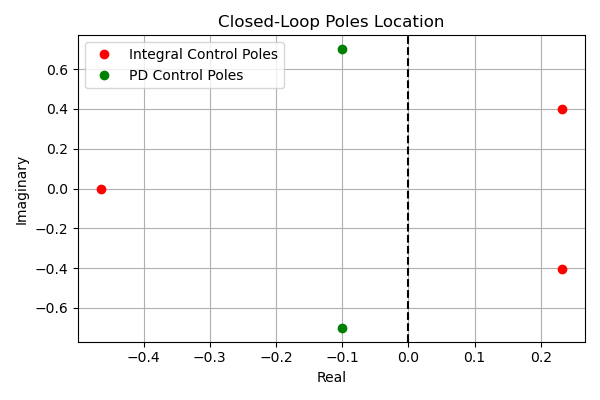
\includegraphics[width=0.90\linewidth]{figs/Controller_Stability.png}
    \caption{Controller Stability}
    \label{fig:EC2025-17-controller-stability}
\end{figure}

\item
Consider the polynomial $p\brak{s}=s^5+7s^4+3s^3-33s^2+2s-40$. Let $\brak{L,I,R}$ be defined as: $L$ is the number of roots of $p\brak{s}$ with negative real parts, $I$ is the number of purely imaginary roots, and $R$ is the number of roots with positive real parts. Which one of the following is correct?
\hfill (EC~2025)
\begin{enumerate}
	\begin{multicols}{2}
    \item $L=2$, $I=2$, and $R=1$
    \item $L=3$, $I=2$, and $R=0$
    \item $L=1$, $I=2$, and $R=2$
    \item $L=0$, $I=4$, and $R=1$
    \end{multicols}
\end{enumerate}
\solution
\begin{align}
\brak{s+5}\brak{s+4}&=s^2+9s+20
\\
\brak{s^2+9s+20}\brak{s-2}&=s^3+7s^2+2s-40
\\
\brak{s^3+7s^2+2s-40}\brak{s^2+1}&=s^5+7s^4+3s^3-33s^2+2s-40
\\
\implies p\brak{s}&=\brak{s+5}\brak{s+4}\brak{s-2}\brak{s^2+1}
\end{align}
The roots $-5,-4$ have negative real parts, $\pm\j$ are purely imaginary and $2$ has a positive real part, so
\begin{align}
\brak{L,I,R}&=\brak{2,2,1}
\end{align}

The following code verifies the solution through a plot
\begin{lstlisting}[frame=single, basicstyle=\rmfamily, escapeinside={(*@}{@*)}]
(*@\makebox[\dimexpr\linewidth-2\fboxsep-2\fboxrule\relax][c]{\texttt{\detokenize{codes/Poly_Roots.py}}}@*)
\end{lstlisting}
\begin{figure}[H]
    \centering
    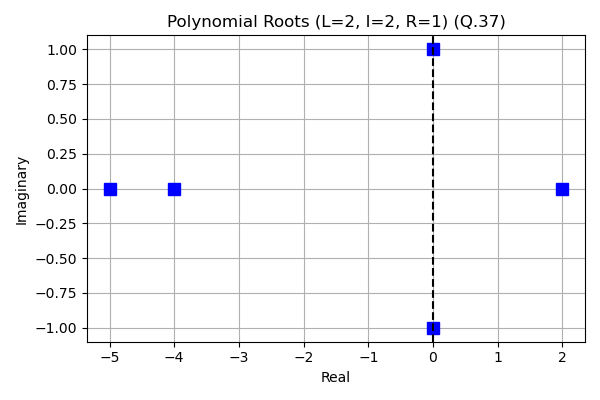
\includegraphics[width=0.90\linewidth]{figs/Poly_Roots.png}
    \caption{Poly Roots}
    \label{fig:EC2025-18-poly-roots}
\end{figure}

\item
Consider a continuous-time finite-energy signal $f\brak{t}$ whose Fourier transform vanishes outside $\sbrak{-\omega_c,\omega_c}$ ($\omega_c$ in rad/s). It is uniformly sampled to obtain $y\brak{t}=f\brak{t}p\brak{t}$, where
\begin{align}
p\brak{t}=\sum_{n=-\infty}^{\infty}\delta\brak{t-\tau-nT_s},\quad T_s>0,\ \tau>0
\end{align}
and $\delta\brak{t}$ is the Dirac impulse. The sampled signal $y\brak{t}$ is passed through an ideal lowpass filter
\begin{align}
h\brak{t}=\omega_cT_s\frac{\sin\brak{\omega_ct}}{\pi\omega_ct}
\end{align}
with cutoff frequency $\omega_c$ and passband gain $T_s$. The output of the filter is \underline{\hspace{1cm}}.
\hfill (EC~2025)
\begin{enumerate}
	\begin{multicols}{2}
    \item $f\brak{t}$ if $T_s<\frac{\pi}{\omega_c}$
    \item $f\brak{t-\tau}$ if $T_s<\frac{\pi}{\omega_c}$
    \item $f\brak{t-\tau}$ if $T_s<\frac{2\pi}{\omega_c}$
    \item $T_sf\brak{t}$ if $T_s<\frac{2\pi}{\omega_c}$
    \end{multicols}
\end{enumerate}
\solution
From \eqref{eq:F-sampled},
\begin{align}
Y\brak{\omega}&=\frac{1}{T_s}\sum_{k}e^{-\j k\omega_s\tau}F\brak{\omega-k\omega_s}
\end{align}
From \eqref{eq:F-nyquist}, the replicas do not overlap if
\begin{align}
\omega_s=\frac{2\pi}{T_s}&>2\omega_c
\\
\iff T_s&<\frac{\pi}{\omega_c}
\end{align}
From \eqref{eq:F-lpf}, only $k=0$ is kept,
\begin{align}
H\brak{\omega}Y\brak{\omega}&=T_s\cdot\frac{1}{T_s}F\brak{\omega}
\\
&=F\brak{\omega}
\end{align}
so the output is $f\brak{t}$.

The following code verifies the solution through a plot
\begin{lstlisting}[frame=single, basicstyle=\rmfamily, escapeinside={(*@}{@*)}]
(*@\makebox[\dimexpr\linewidth-2\fboxsep-2\fboxrule\relax][c]{\texttt{\detokenize{codes/Sampling_Reconstruction.py}}}@*)
\end{lstlisting}
\begin{figure}[H]
    \centering
    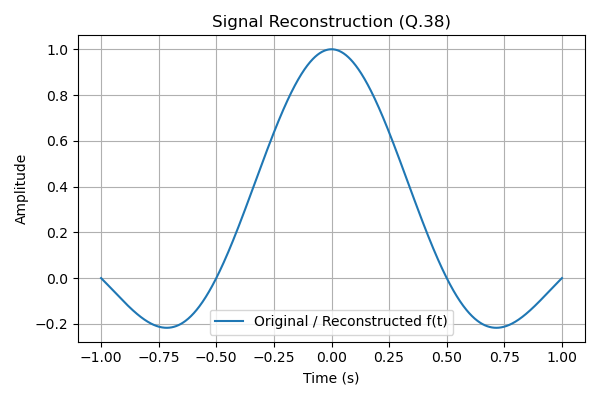
\includegraphics[width=0.90\linewidth]{figs/Sampling_Reconstruction.png}
    \caption{Sampling Reconstruction}
    \label{fig:EC2025-19-sampling-reconstruction}
\end{figure}

\item
In the circuit of the given circuit, $M_1$ is an ideal AC voltmeter and $M_2$ is an ideal AC ammeter. The source voltage (in Volts) is $v_s\brak{t}=100\cos\brak{200t}$. What should be the value of the variable capacitor $C$ such that the RMS readings on $M_1$ and $M_2$ are 25 V and 5 A, respectively?
\hfill (EC~2025)
\begin{enumerate}
	\begin{multicols}{2}
    \item $25\ \mu$F
    \item $4\ \mu$F
    \item $0.25\ \mu$F
    \item Insufficient information to find $C$
    \end{multicols}
\end{enumerate}


\begin{figure}[H]
    \centering
    \begin{tikzpicture}[font=\footnotesize,>=Stealth]
      % voltage source
      \draw (0,0)--(0,1);
      \draw (0,2)--(0,3);
      \draw (0,1.5) circle (0.5);
      \draw (-0.3,1.5) sin (-0.15,1.7) cos (0,1.5) sin (0.15,1.3) cos (0.3,1.5);
      \node at (0.33,2.3) {$+$};
      \node at (0.33,0.7) {$-$};
      \node[left] at (-0.6,1.5) {$v_s(t)$};
      % LTI box
      \draw (0,3)--(1,3);
      \draw (0,0)--(1,0);
      \draw (1,-0.3) rectangle (2.8,3.3);
      \node[align=center,text width=1.5cm] at (1.9,1.5) {Linear Time Invariant Circuit};
      % top and bottom wires to the right of the box
      \draw (2.8,3)--(4.6,3);
      \draw (2.8,0)--(6.4,0);
      \fill (3.8,3) circle (1.2pt);
      \fill (3.8,0) circle (1.2pt);
      % voltmeter M1
      \node[draw,circle,minimum size=0.8cm,inner sep=0pt] (M1) at (3.8,1.5) {$M_1$};
      \draw (3.8,3)--(M1.north);
      \draw (M1.south)--(3.8,0);
      \node at (4.12,2.35) {$+$};
      \node at (4.12,0.65) {$-$};
      % ammeter M2
      \node[draw,circle,minimum size=0.8cm,inner sep=0pt] (M2) at (5.0,3) {$M_2$};
      \draw (M2.east)--(6.4,3)--(6.4,2.8);
      % series branch: 5 ohm, variable C, 1 H
      \draw[decorate,decoration={zigzag,segment length=4pt,amplitude=3pt}] (6.4,2.8)--(6.4,2.0);
      \draw (6.4,2.0)--(6.4,1.65);
      \draw (6.1,1.65)--(6.7,1.65);
      \draw (6.1,1.45)--(6.7,1.45);
      \draw (6.4,1.45)--(6.4,1.2);
      \draw[->] (6.0,1.3)--(6.8,1.85);
      \draw[decorate,decoration={coil,aspect=0.5,segment length=3.5pt,amplitude=3.5pt}] (6.4,1.2)--(6.4,0.35);
      \draw (6.4,0.35)--(6.4,0);
      \node[right] at (6.6,2.4) {$5\,\Omega$};
      \node[right] at (6.85,1.55) {$C$};
      \node[right] at (6.65,0.75) {$1$ H};
    \end{tikzpicture}
    \caption{Circuit with meters $M_1$, $M_2$ and capacitor $C$}
    \label{fig:q39}
\end{figure}

\solution
From the given circuit,
\begin{align}
\abs{Z}&=\frac{V}{I}
\\
&=\frac{25}{5}
\\
&=5\ \Omega
\end{align}
From \eqref{eq:F-series-rlc},
\begin{align}
\sqrt{R^2+\brak{\omega L-\frac{1}{\omega C}}^2}&=R
\\
\implies\omega L&=\frac{1}{\omega C}
\end{align}
From \eqref{eq:F-resonance},
\begin{align}
C&=\frac{1}{\omega^2L}
\\
&=\frac{1}{200^2\times1}
\\
&=25\ \mu\text{F}
\end{align}

The following code verifies the solution through a plot
\begin{lstlisting}[frame=single, basicstyle=\rmfamily, escapeinside={(*@}{@*)}]
(*@\makebox[\dimexpr\linewidth-2\fboxsep-2\fboxrule\relax][c]{\texttt{\detokenize{codes/AC_Meters.py}}}@*)
\end{lstlisting}
\begin{figure}[H]
    \centering
    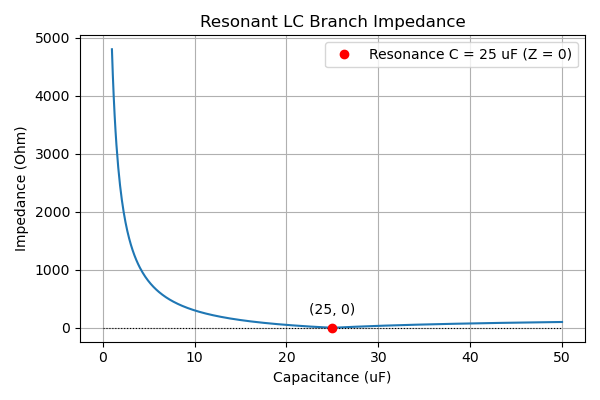
\includegraphics[width=0.90\linewidth]{figs/AC_Meters.png}
    \caption{AC Meters}
    \label{fig:EC2025-20-ac-meters}
\end{figure}

\item
The $Z$-parameter matrix of a two-port network relates port voltages and currents by
\begin{align}
\myvec{V_1\\V_2}=\vec{Z}\myvec{I_1\\I_2}
\end{align}
The $Z$-parameter matrix (each entry in Ohms) of the network in the given network is \underline{\hspace{1cm}}.
\hfill (EC~2025)
\begin{enumerate}
	\begin{multicols}{4}
    \item $\myvec{\frac{10}{3}&\frac{2}{3}\\\frac{2}{3}&\frac{10}{3}}$
    \item $\myvec{\frac{2}{3}&\frac{10}{3}\\\frac{10}{3}&\frac{2}{3}}$
    \item $\myvec{10&2\\2&10}$
    \item $\myvec{\frac{10}{3}&\frac{1}{3}\\\frac{1}{3}&\frac{10}{3}}$
    \end{multicols}
\end{enumerate}


\begin{figure}[H]
    \centering
    \begin{tikzpicture}[font=\footnotesize,>=Stealth,
        zz/.style={decorate,decoration={zigzag,segment length=4pt,amplitude=3pt}}]
      % top rail with series resistors
      \draw (0,2)--(0.5,2);
      \draw[zz] (0.5,2)--(1.4,2);
      \draw (1.4,2)--(3.0,2);
      \draw[zz] (3.0,2)--(3.9,2);
      \draw (3.9,2)--(5.5,2);
      \draw[zz] (5.5,2)--(6.4,2);
      \draw (6.4,2)--(7.0,2);
      % bottom rail
      \draw (0,0)--(7.0,0);
      % shunt resistors
      \draw (2.2,2)--(2.2,1.45);
      \draw[zz] (2.2,1.45)--(2.2,0.55);
      \draw (2.2,0.55)--(2.2,0);
      \draw (4.7,2)--(4.7,1.45);
      \draw[zz] (4.7,1.45)--(4.7,0.55);
      \draw (4.7,0.55)--(4.7,0);
      % dots
      \foreach \p in {(0,2),(0,0),(7,2),(7,0),(2.2,2),(2.2,0),(4.7,2),(4.7,0)}
        \fill \p circle (1.5pt);
      % resistor labels
      \node at (0.95,1.6) {$2\,\Omega$};
      \node at (3.45,1.6) {$2\,\Omega$};
      \node at (5.95,1.6) {$2\,\Omega$};
      \node[right] at (2.35,1.0) {$2\,\Omega$};
      \node[right] at (4.85,1.0) {$2\,\Omega$};
      % currents
      \draw[->] (0.15,2.3)--(0.75,2.3);
      \node at (0.45,2.55) {$I_1$};
      \draw[->] (6.85,2.3)--(6.25,2.3);
      \node at (6.55,2.55) {$I_2$};
      % port voltages
      \draw[<->] (-0.35,0.15)--(-0.35,1.85);
      \node[left] at (-0.4,1.0) {$V_1$};
      \node at (-0.6,1.7) {$+$};
      \node at (-0.6,0.3) {$-$};
      \draw[<->] (7.35,0.15)--(7.35,1.85);
      \node[right] at (7.4,1.0) {$V_2$};
      \node at (7.6,1.7) {$+$};
      \node at (7.6,0.3) {$-$};
    \end{tikzpicture}
    \caption{Two-port network}
    \label{fig:q40}
\end{figure}

\solution
With port 2 open, from \eqref{eq:F-rnet},
\begin{align}
R_A&=2\parallel\brak{2+2}
\\
&=\frac{2\cdot4}{2+4}
\\
&=\frac{4}{3}\ \Omega
\end{align}
From \eqref{eq:F-zparam},
\begin{align}
z_{11}&=2+R_A
\\
&=\frac{10}{3}\ \Omega
\\
V_2&=\frac{2}{2+2}I_1R_A
\\
&=\frac{2}{3}I_1
\\
z_{21}&=\frac{2}{3}\ \Omega
\end{align}
The network is reciprocal and symmetric, so from \eqref{eq:F-zdef},
\begin{align}
\vec{Z}&=\myvec{\frac{10}{3}&\frac{2}{3}\\\frac{2}{3}&\frac{10}{3}}\ \Omega
\end{align}

The following code verifies the solution through a plot
\begin{lstlisting}[frame=single, basicstyle=\rmfamily, escapeinside={(*@}{@*)}]
(*@\makebox[\dimexpr\linewidth-2\fboxsep-2\fboxrule\relax][c]{\texttt{\detokenize{codes/Opamp_Gain.py}}}@*)
\end{lstlisting}
\begin{figure}[H]
    \centering
    \includegraphics[width=0.90\linewidth]{figs/Opamp_Gain.png}
    \caption{Opamp Gain}
    \label{fig:EC2025-21-opamp-gain}
\end{figure}

\item
A source transmits a symbol $S$ taking values uniformly at random from $\cbrak{-2,0,2}$. The receiver obtains $Y=S+N$, where $N$ is a zero-mean Gaussian random variable independent of $S$, and uses the maximum-likelihood decoder. Suppose the probability of symbol error is $P_e=\alpha\pr{N>1}$. What is $\alpha$?
\hfill (EC~2025)
\begin{enumerate}
	\begin{multicols}{4}
    \item $\frac{1}{3}$
    \item $1$
    \item $\frac{2}{3}$
    \item $\frac{4}{3}$
    \end{multicols}
\end{enumerate}
\solution
From \eqref{eq:F-ml}, the decision boundaries are $-1$ and $1$. Let $p=\pr{N>1}$. From \eqref{eq:F-gauss-sym},
\begin{align}
\pr{\text{error}|S=-2}&=\pr{N>1}=p
\\
\pr{\text{error}|S=0}&=\pr{\abs{N}>1}=2p
\\
\pr{\text{error}|S=2}&=\pr{N<-1}=p
\\
P_e&=\frac{1}{3}\brak{p+2p+p}
\\
&=\frac{4}{3}p
\end{align}
so $\alpha=\frac{4}{3}$.

The following code verifies the solution through a plot
\begin{lstlisting}[frame=single, basicstyle=\rmfamily, escapeinside={(*@}{@*)}]
(*@\makebox[\dimexpr\linewidth-2\fboxsep-2\fboxrule\relax][c]{\texttt{\detokenize{codes/Smith_Chart.py}}}@*)
\end{lstlisting}
\begin{figure}[H]
    \centering
    \includegraphics[width=0.90\linewidth]{figs/Smith_Chart.png}
    \caption{Smith Chart}
    \label{fig:EC2025-22-smith-chart}
\end{figure}

\item
Consider the real-valued random process
\begin{align}
f\brak{t}=\sum_{n=1}^{N}a_np\brak{t-nT}
\end{align}
where $T>0$, $N$ is a positive integer, $p\brak{t}=1$ for $t\in\sbrak{0,0.5T}$ and $0$ otherwise, and the coefficients $a_n$ are pairwise independent, zero-mean, unit-variance random variables. Consider:
\\
(i) The mean of the process $f\brak{t}$ is independent of time $t$.
\\
(ii) The autocorrelation $E\sbrak{f\brak{t}f\brak{t+\tau}}$ is independent of $t$ for all $\tau$.
\\
Choose the correct option.
\hfill (EC~2025)
\begin{enumerate}
	\begin{multicols}{2}
    \item (i) is TRUE and (ii) is FALSE
    \item Both (i) and (ii) are TRUE
    \item Both (i) and (ii) are FALSE
    \item (i) is FALSE and (ii) is TRUE
    \end{multicols}
\end{enumerate}
\solution
From \eqref{eq:F-expect},
\begin{align}
E\sbrak{f\brak{t}}&=\sum_{n=1}^{N}E\sbrak{a_n}p\brak{t-nT}
\\
&=0
\end{align}
so (i) is true. From \eqref{eq:F-uncorr},
\begin{align}
E\sbrak{f\brak{t}f\brak{t+\tau}}&=\sum_{n=1}^{N}p\brak{t-nT}p\brak{t+\tau-nT}
\end{align}
For $\tau=0$,
\begin{align}
E\sbrak{f\brak{t}^2}&=\sum_{n=1}^{N}p\brak{t-nT}
\\
&\in\cbrak{0,1}
\end{align}
which depends on $t$, so (ii) is false.

The following code verifies the solution.
\begin{lstlisting}[frame=single, basicstyle=\rmfamily, escapeinside={(*@}{@*)}]
(*@\makebox[\dimexpr\linewidth-2\fboxsep-2\fboxrule\relax][c]{\texttt{\detokenize{codes/Wave_Propagation.c}}}@*)
\end{lstlisting}

\item
A 10-bit analog-to-digital converter (ADC) has a sampling frequency of 1 MHz and a full-scale voltage of 3.3 V. For an input sinusoid of frequency 500 kHz, the maximum SNR (in dB, two decimal places) and the data rate (in Mbps) at the ADC output are \underline{\hspace{1cm}}, respectively.
\hfill (EC~2025)
\begin{enumerate}
	\begin{multicols}{4}
    \item 61.96 and 10
    \item 61.96 and 5
    \item 33.36 and 10
    \item 33.36 and 5
    \end{multicols}
\end{enumerate}
\solution
From \eqref{eq:F-adc}, for $N=10$ and $f_s=1$ MHz,
\begin{align}
\text{SNR}_{\max}&=6.02\brak{10}+1.76
\\
&=61.96\text{ dB}
\\
R_b&=f_sN
\\
&=\brak{10^6}\brak{10}
\\
&=10\text{ Mbps}
\end{align}

The following code verifies the solution through a plot
\begin{lstlisting}[frame=single, basicstyle=\rmfamily, escapeinside={(*@}{@*)}]
(*@\makebox[\dimexpr\linewidth-2\fboxsep-2\fboxrule\relax][c]{\texttt{\detokenize{codes/PN_Junction.py}}}@*)
\end{lstlisting}
\begin{figure}[H]
    \centering
    \includegraphics[width=0.90\linewidth]{figs/PN_Junction.png}
    \caption{PN Junction}
    \label{fig:EC2025-24-pn-junction}
\end{figure}

\item
A positive-edge-triggered sequential circuit is shown in the given sequential circuit and timing diagram. There are no timing violations. Input $P_0$ is logic `0' and $P_1$ is logic `1' at all times. The timing diagram of $SEL$ and $S$ is also shown. The sequence of output $Y$ from time $T_0$ to $T_3$ is \underline{\hspace{1cm}}.
\hfill (EC~2025)
\begin{enumerate}
	\begin{multicols}{4}
    \item 1011
    \item 0100
    \item 0010
    \item 1101
    \end{multicols}
\end{enumerate}


\begin{figure}[H]
    \centering
    \resizebox{\linewidth}{!}{%
    \begin{tikzpicture}[font=\footnotesize,>=Stealth]
      % ---------- MUX 1 ----------
      \begin{scope}[shift={(0,0.4)}]
        \draw (0,1)--(0.9,0.6)--(0.9,-0.6)--(0,-1)--cycle;
        \node at (0.17,0.6) {\scriptsize $1$};
        \node at (0.17,-0.6) {\scriptsize $0$};
      \end{scope}
      \draw (-0.6,1.0)--(0,1.0);
      \node[left] at (-0.6,1.0) {$S$};
      \draw (-0.6,-0.2)--(0,-0.2);
      \node[left] at (-0.6,-0.2) {$P0$};
      \draw (0.45,-0.4)--(0.45,-1.1);
      \node at (0.45,-1.35) {$SEL$};
      \draw[->] (0.9,0.4)--(2.0,0.4);
      % ---------- FF 1 ----------
      \draw (2.0,-0.8) rectangle (3.2,0.8);
      \node at (2.2,0.4) {$D$};
      \node at (3.0,0.4) {$Q$};
      \node at (3.0,-0.4) {$\overline{Q}$};
      \draw (2.45,-0.8)--(2.6,-0.58)--(2.75,-0.8);
      \draw (2.6,-0.8)--(2.6,-1.5);
      \node at (2.6,-1.75) {$CLK$};
      % Q1 to MUX 2 input 1
      \draw (3.2,0.4)--(3.8,0.4)--(3.8,1.0)--(4.6,1.0);
      % ---------- MUX 2 ----------
      \begin{scope}[shift={(4.6,0.4)}]
        \draw (0,1)--(0.9,0.6)--(0.9,-0.6)--(0,-1)--cycle;
        \node at (0.17,0.6) {\scriptsize $1$};
        \node at (0.17,-0.6) {\scriptsize $0$};
      \end{scope}
      \node at (4.0,-0.2) {$P1$};
      \draw (4.25,-0.2)--(4.6,-0.2);
      \draw (5.05,-0.4)--(5.05,-1.1);
      \node at (5.05,-1.35) {$SEL$};
      \draw[->] (5.5,0.4)--(6.4,0.4);
      % ---------- FF 2 ----------
      \draw (6.4,-0.8) rectangle (7.6,0.8);
      \node at (6.6,0.4) {$D$};
      \node at (7.4,0.4) {$Q$};
      \node at (7.4,-0.4) {$\overline{Q}$};
      \draw (6.85,-0.8)--(7.0,-0.58)--(7.15,-0.8);
      \draw (7.0,-0.8)--(7.0,-1.5);
      \node at (7.0,-1.75) {$CLK$};
      \draw (7.6,0.4)--(8.0,0.4);
      % ---------- XOR gate ----------
      \begin{scope}[shift={(8.9,-2.2)}]
        \draw (0,0.4) .. controls (0.5,0.4) and (0.8,0.2) .. (0.95,0);
        \draw (0.95,0) .. controls (0.8,-0.2) and (0.5,-0.4) .. (0,-0.4);
        \draw (0,-0.4) .. controls (0.2,-0.15) and (0.2,0.15) .. (0,0.4);
        \draw (-0.12,-0.4) .. controls (0.08,-0.15) and (0.08,0.15) .. (-0.12,0.4);
      \end{scope}
      \draw (7.6,-0.4)--(8.4,-0.4)--(8.4,-2.0)--(9.0,-2.0);
      \draw (3.2,-0.4)--(3.55,-0.4)--(3.55,-2.4)--(9.0,-2.4);
      \draw (9.85,-2.2)--(10.5,-2.2);
      \node[right] at (10.5,-2.2) {$Y$};
      % ---------- timing diagram ----------
      \begin{scope}[shift={(2.2,-6.2)}]
        \foreach \x/\l in {1/0,2/1,3/2,4/3} {
          \draw[dashed] (\x,2.5)--(\x,-0.5);
          \node at (\x,-0.8) {$T_{\l}$};
        }
        \draw[thick] (0,1.8)--(0.5,1.8)--(0.5,2.2)--(1,2.2)--(1,1.8)--(1.5,1.8)--(1.5,2.2)--(2,2.2)--(2,1.8)--(2.5,1.8)--(2.5,2.2)--(3,2.2)--(3,1.8)--(3.5,1.8)--(3.5,2.2)--(4,2.2)--(4,1.8)--(4.6,1.8);
        \draw[thick] (0,0.9)--(1.27,0.9)--(1.27,1.3)--(3.23,1.3)--(3.23,0.9)--(4.6,0.9);
        \draw[thick] (0,0)--(2.3,0)--(2.3,0.4)--(4.25,0.4)--(4.25,0)--(4.6,0);
        \node[left] at (0,2.0) {$CLK$};
        \node[left] at (0,1.1) {$SEL$};
        \node[left] at (0,0.2) {$S$};
      \end{scope}
    \end{tikzpicture}}
    \caption{Positive-edge-triggered sequential circuit and input timing}
    \label{fig:q45}
\end{figure}

\solution
From the given sequential circuit and timing diagram and \eqref{eq:F-dff},
\begin{align}
Q_1^{+}&=\begin{cases}S,&SEL=1\\0,&SEL=0\end{cases}
\\
Q_2^{+}&=\begin{cases}Q_1,&SEL=1\\1,&SEL=0\end{cases}
\\
Y&=\overline{Q_1}\oplus\overline{Q_2}
\\
&=Q_1\oplus Q_2
\end{align}
Reading $SEL$ and $S$ at the rising edges before $T_0,\dots,T_3$,
\begin{center}
\begin{tabular}{|c|c|c|c|c|c|}
\hline
edge before&$SEL$&$S$&$Q_1$&$Q_2$&$Y$\\
\hline
$T_0$&0&0&0&1&1\\
$T_1$&1&0&0&0&0\\
$T_2$&1&1&1&0&1\\
$T_3$&0&1&0&1&1\\
\hline
\end{tabular}
\end{center}
The output sequence is $Y=1011$.

The following code verifies the solution through a plot
\begin{lstlisting}[frame=single, basicstyle=\rmfamily, escapeinside={(*@}{@*)}]
(*@\makebox[\dimexpr\linewidth-2\fboxsep-2\fboxrule\relax][c]{\texttt{\detokenize{codes/MOSFET_Characteristics.py}}}@*)
\end{lstlisting}
\begin{figure}[H]
    \centering
    \includegraphics[width=0.90\linewidth]{figs/MOSFET_Characteristics.png}
    \caption{MOSFET Characteristics}
    \label{fig:EC2025-25-mosfet-characteristics}
\end{figure}

\item
A square metal sheet of $4\text{ m}\times4\text{ m}$ is placed on the $x$--$y$ plane as in the given sheet geometry. If the surface charge density (in $\mu$C/m$^2$) is $\rho_s\brak{x,y}=4\abs{y}$, the total charge (in $\mu$C, rounded off to the nearest integer) on the sheet is \underline{\hspace{1cm}}.
\hfill (EC~2025)
\begin{enumerate}
	\begin{multicols}{4}
    \item 16
    \item 85
    \item 64
    \item 256
    \end{multicols}
\end{enumerate}


\begin{figure}[H]
    \centering
    \begin{tikzpicture}[x=0.8cm,y=0.8cm,font=\footnotesize,>=Stealth]
      \fill[pattern=north east lines,pattern color=gray] (-2,-2) rectangle (2,2);
      \draw (-2,-2) rectangle (2,2);
      \draw[->] (-3.2,0)--(3.2,0) node[right] {$x$ (m)};
      \draw[->] (0,-2.8)--(0,3.1) node[above] {$y$ (m)};
      \node[above left] at (-2,2) {$(-2,2)$};
      \node[above right] at (2,2) {$(2,2)$};
      \node[below left] at (-2,-2) {$(-2,-2)$};
      \node[below right] at (2,-2) {$(2,-2)$};
    \end{tikzpicture}
    \caption{Square metal sheet on the $x$-$y$ plane}
    \label{fig:q49}
\end{figure}

\solution
From the given sheet geometry, the sheet is $-2\le x\le2$, $-2\le y\le2$. From \eqref{eq:F-charge},
\begin{align}
Q&=\int_{-2}^{2}\int_{-2}^{2}4\abs{y}\,dx\,dy
\\
&=4\brak{\int_{-2}^{2}dx}\brak{2\int_{0}^{2}y\,dy}
\\
&=4\cdot4\cdot4
\\
&=64\ \mu\text{C}
\end{align}

The following code verifies the solution.
\begin{lstlisting}[frame=single, basicstyle=\rmfamily, escapeinside={(*@}{@*)}]
(*@\makebox[\dimexpr\linewidth-2\fboxsep-2\fboxrule\relax][c]{\texttt{\detokenize{codes/Counter_Sync.c}}}@*)
\end{lstlisting}

\item
An electric field of $0.01$ V/m is applied along the length of a copper wire of circular cross-section with diameter 1 mm. Copper has conductivity $5.8\times10^7$ S/m. The current (in Amperes, two decimal places) through the wire is \underline{\hspace{1cm}}.
\hfill (EC~2025)
\begin{enumerate}
	\begin{multicols}{4}
    \item 0.46
    \item 1.82
    \item 0.58
    \item 1.12
    \end{multicols}
\end{enumerate}
\solution
From \eqref{eq:F-J}, with $r=0.5$ mm,
\begin{align}
J&=\sigma E
\\
&=\brak{5.8\times10^7}\brak{0.01}
\\
&=5.8\times10^5\text{ A/m}^2
\\
I&=JA
\\
&=5.8\times10^5\cdot\pi\brak{5\times10^{-4}}^2
\\
&=0.4555\text{ A}
\\
&\approx0.46\text{ A}
\end{align}

The following code verifies the solution through a plot
\begin{lstlisting}[frame=single, basicstyle=\rmfamily, escapeinside={(*@}{@*)}]
(*@\makebox[\dimexpr\linewidth-2\fboxsep-2\fboxrule\relax][c]{\texttt{\detokenize{codes/Laplace_ROC.py}}}@*)
\end{lstlisting}
\begin{figure}[H]
    \centering
    \includegraphics[width=0.90\linewidth]{figs/Laplace_ROC.png}
    \caption{Laplace ROC}
    \label{fig:EC2025-27-laplace-roc}
\end{figure}

\item
Consider a non-negative function $f\brak{x}$, continuous and bounded on $\sbrak{2,8}$. Let $M$ and $m$ be its maximum and minimum on the interval. Choose the combination(s) of $\alpha$ and $\beta$ for which
\begin{align}
\beta\le\int_{2}^{8}f\brak{x}\,dx\le\alpha
\end{align}
is guaranteed to hold.
\hfill (EC~2025)
\begin{enumerate}
	\begin{multicols}{2}
    \item $\beta=5m$, $\alpha=7M$
    \item $\beta=6m$, $\alpha=5M$
    \item $\beta=7m$, $\alpha=6M$
    \item $\beta=7m$, $\alpha=5M$
    \end{multicols}
\end{enumerate}
\solution
From \eqref{eq:F-intbound}, with $b-a=6$,
\begin{align}
6m\le\int_{2}^{8}f\brak{x}\,dx\le6M
\end{align}
The inequality is guaranteed when $\beta\le6m$ and $\alpha\ge6M$. Only (A) satisfies
\begin{align}
5m&\le6m
\\
7M&\ge6M
\end{align}

The following code verifies the solution through a plot
\begin{lstlisting}[frame=single, basicstyle=\rmfamily, escapeinside={(*@}{@*)}]
(*@\makebox[\dimexpr\linewidth-2\fboxsep-2\fboxrule\relax][c]{\texttt{\detokenize{codes/ADC_Performance.py}}}@*)
\end{lstlisting}
\begin{figure}[H]
    \centering
    
\includegraphics[width=0.90\linewidth]{figs/ADC_Performance.png}
    \caption{ADC Performance}
    \label{fig:EC2025-28-adc-performance}
\end{figure}

\item
Which of the following statements about contour integrals (counter-clockwise) on the unit circle $C$ in the complex plane is/are TRUE?
\hfill (EC~2025)
\begin{enumerate}
	\begin{multicols}{2}
    \item $\oint_Ce^z\,dz=0$
    \item $\oint_Cz^n\,dz=0$, where $n$ is an even integer
    \item $\oint_C\cos z\,dz\neq0$
    \item $\oint_C\sec z\,dz\neq0$
    \end{multicols}
\end{enumerate}
\solution
$e^z$ and $\cos z$ are analytic everywhere. From \eqref{eq:F-cauchy},
\begin{align}
\oint_Ce^z\,dz&=0
\\
\oint_C\cos z\,dz&=0
\end{align}
so (A) is true and (C) is false. From \eqref{eq:F-zn}, for even $n$,
\begin{align}
\oint_Cz^n\,dz&=0
\end{align}
so (B) is true. From \eqref{eq:F-sec}, the poles of $\sec z$ lie outside $\abs{z}=1$, so from \eqref{eq:F-cauchy},
\begin{align}
\oint_C\sec z\,dz&=0
\end{align}
and (D) is false.

The following code verifies the solution through a plot
\begin{lstlisting}[frame=single, basicstyle=\rmfamily, escapeinside={(*@}{@*)}]
(*@\makebox[\dimexpr\linewidth-2\fboxsep-2\fboxrule\relax][c]{\texttt{\detokenize{codes/Signal_Flow_Graph.py}}}@*)
\end{lstlisting}
\begin{figure}[H]
    \centering
    
\includegraphics[width=0.90\linewidth]{figs/Signal_Flow_Graph.png}
    \caption{Signal Flow Graph}
    \label{fig:EC2025-29-signal-flow-graph}
\end{figure}

\item
Consider a system with internal states $x_1\brak{t},x_2\brak{t},x_3\brak{t}$ and input $u\brak{t}$ governed by
\begin{align}
\frac{d}{dt}\myvec{x_1\\x_2\\x_3}=\myvec{2&0&0\\0&-2&0\\0&0&0}\myvec{x_1\\x_2\\x_3}+\myvec{1\\1\\1}u\brak{t}
\end{align}
Which of the following statements is/are TRUE?
\hfill (EC~2025)
\begin{enumerate}
    \item The signals $x_1,x_2,x_3$ are bounded for all bounded inputs.
    \item There exists a bounded input such that at least one of $x_1,x_2,x_3$ is unbounded.
    \item There exists a bounded input such that the signals $x_1,x_2,x_3$ are unbounded.
    \item The signals $x_1,x_2,x_3$ are unbounded for all bounded inputs.
\end{enumerate}
\solution
The states decouple,
\begin{align}
\dot{x}_1&=2x_1+u
\\
\dot{x}_2&=-2x_2+u
\\
\dot{x}_3&=u
\end{align}
For $u\equiv1$ and zero initial state, from \eqref{eq:F-state-unbounded}, \eqref{eq:F-state-integrator} and \eqref{eq:F-state-bounded},
\begin{align}
x_1\brak{t}&=\frac{1}{2}\brak{e^{2t}-1}\to\infty
\\
x_3\brak{t}&=t\to\infty
\\
\abs{x_2\brak{t}}&\le\abs{x_2\brak{0}}+\frac{U}{2}
\end{align}
So (B) is true, while (A), (C) and (D) are false.

The following code verifies the solution through a plot
\begin{lstlisting}[frame=single, basicstyle=\rmfamily, escapeinside={(*@}{@*)}]
(*@\makebox[\dimexpr\linewidth-2\fboxsep-2\fboxrule\relax][c]{\texttt{\detokenize{codes/Noise_PSD.py}}}@*)
\end{lstlisting}
\begin{figure}[H]
    \centering
    \includegraphics[width=0.90\linewidth]{figs/Noise_PSD.png}
    \caption{Noise PSD}
    \label{fig:EC2025-30-noise-psd}
\end{figure}

\item
The random variable $X$ takes values in $\cbrak{-1,0,1}$ with $\pr{X=-1}=\pr{X=1}=\alpha$ and $\pr{X=0}=1-2\alpha$, where $0<\alpha<\frac{1}{2}$. Let $g\brak{\alpha}$ be the entropy of $X$ in bits. Which of the following is/are TRUE?
\hfill (EC~2025)
\begin{enumerate}
	\begin{multicols}{2}
    \item $g\brak{0.4}>g\brak{0.3}$
    \item $g\brak{0.3}>g\brak{0.4}$
    \item $g\brak{0.3}>g\brak{0.25}$
    \item $g\brak{0.25}>g\brak{0.3}$
    \end{multicols}
\end{enumerate}
\solution
From \eqref{eq:F-entropy},
\begin{align}
g\brak{\alpha}&=-2\alpha\log_2\alpha-\brak{1-2\alpha}\log_2\brak{1-2\alpha}
\\
g^{\prime}\brak{\alpha}&=2\log_2\frac{1-2\alpha}{\alpha}
\end{align}
$g^{\prime}>0$ for $\alpha<\frac{1}{3}$. Evaluating,
\begin{align}
g\brak{0.25}&=1.5000
\\
g\brak{0.3}&=1.5710
\\
g\brak{0.4}&=1.5219
\end{align}
Hence (B) and (C) are true.

The following code verifies the solution.
\begin{lstlisting}[frame=single, basicstyle=\rmfamily, escapeinside={(*@}{@*)}]
(*@\makebox[\dimexpr\linewidth-2\fboxsep-2\fboxrule\relax][c]{\texttt{\detokenize{codes/BPSK_BER.c}}}@*)
\end{lstlisting}

\item
Let $f\brak{t}$ be periodic with fundamental period $T_0>0$, and $y\brak{t}=f\brak{\alpha t}$ with $\alpha>1$. Their Fourier series are
\begin{align}
f\brak{t}&=\sum_{k=-\infty}^{\infty}c_ke^{\j\frac{2\pi}{T_0}kt}
\\
y\brak{t}&=\sum_{k=-\infty}^{\infty}d_ke^{\j\frac{2\pi\alpha}{T_0}kt}
\end{align}
Which of the following is/are TRUE?
\hfill (EC~2025)
\begin{enumerate}
	\begin{multicols}{2}
    \item $c_k=d_k$ for all $k$
    \item $y\brak{t}$ is periodic with fundamental period $\alpha T_0$
    \item $c_k=\frac{d_k}{\alpha}$ for all $k$
    \item $y\brak{t}$ is periodic with fundamental period $\frac{T_0}{\alpha}$
    \end{multicols}
\end{enumerate}
\solution
From \eqref{eq:F-fs-period},
\begin{align}
y\brak{t+\frac{T_0}{\alpha}}&=f\brak{\alpha t+T_0}
\\
&=y\brak{t}
\end{align}
so the period is $\frac{T_0}{\alpha}$. From \eqref{eq:F-fs-scale},
\begin{align}
y\brak{t}&=\sum_{k}c_ke^{\j\frac{2\pi k\alpha t}{T_0}}
\\
\implies d_k&=c_k
\end{align}
Hence (A) and (D) are true.

The following code verifies the solution through a plot
\begin{lstlisting}[frame=single, basicstyle=\rmfamily, escapeinside={(*@}{@*)}]
(*@\makebox[\dimexpr\linewidth-2\fboxsep-2\fboxrule\relax][c]{\texttt{\detokenize{codes/Antenna_Pattern.py}}}@*)
\end{lstlisting}
\begin{figure}[H]
    \centering
    \includegraphics[width=0.90\linewidth]{figs/Antenna_Pattern.png}
    \caption{Antenna Pattern}
    \label{fig:EC2025-32-antenna-pattern}
\end{figure}

\item
Consider the system represented by the block diagram in the given block diagram. Which of the signal flow graphs in the given signal-flow graphs represent(s) this system? Choose the correct option(s).
\hfill (EC~2025)
\begin{enumerate}
	\begin{multicols}{4}
    \item graph (A)
    \item graph (B)
    \item graph (C)
    \item graph (D)
    \end{multicols}
\end{enumerate}


\begin{figure}[H]
    \centering
    \begin{tikzpicture}[font=\footnotesize,>=Stealth,
        blk/.style={draw,minimum width=1cm,minimum height=0.7cm,inner sep=3pt},
        sm/.style={draw,circle,minimum size=0.6cm,inner sep=0pt}]
      \node (R) at (-1.7,0) {$R(s)$};
      \node[sm] (s1) at (0,0) {};
      \draw (s1.north west)--(s1.south east);
      \draw (s1.north east)--(s1.south west);
      \node[blk] (G1) at (2.4,0) {$G_1$};
      \node[blk] (G2) at (2.4,1.4) {$G_2$};
      \node[sm] (s2) at (4.8,0) {};
      \draw (s2.north west)--(s2.south east);
      \draw (s2.north east)--(s2.south west);
      \node (Y) at (6.4,0) {$Y(s)$};
      \draw[->] (R.east)--(s1.west);
      \draw[->] (s1.east)--(G1.west);
      \draw[->] (G1.east)--(s2.west);
      \draw[->] (s2.east)--(Y.west);
      \fill (1.0,0) circle (1.2pt);
      \fill (3.7,0) circle (1.2pt);
      % G2 path
      \draw (1.0,0)--(1.0,1.4);
      \draw[->] (1.0,1.4)--(G2.west);
      \draw (G2.east)--(4.8,1.4);
      \draw[->] (4.8,1.4)--(s2.north);
      % feedback
      \draw[->] (3.7,0)--(3.7,-1.2)--(0,-1.2)--(s1.south);
      \node at ($(s1.west)+(-0.25,0.22)$) {$+$};
      \node at ($(s1.south)+(0.25,-0.25)$) {$-$};
      \node at ($(s2.west)+(-0.25,0.22)$) {$+$};
      \node at ($(s2.north)+(0.25,0.25)$) {$+$};
    \end{tikzpicture}
    \caption{Block diagram of the system}
    \label{fig:q56}
\end{figure}

\begin{figure}[H]
    \centering
    \resizebox{\linewidth}{!}{%
    \begin{tikzpicture}[font=\footnotesize,>=Stealth,
        nd/.style={circle,draw,fill=white,inner sep=1.3pt}]
      % ---------- (A) ----------
      \begin{scope}[shift={(0,0)}]
        \node[nd] (a0) at (0,0) {};
        \node[nd] (a1) at (1.0,0) {};
        \node[nd] (a2) at (2.2,0) {};
        \node[nd] (a3) at (3.2,0) {};
        \node[anchor=east] at (-0.12,0) {$R(s)$};
        \node[anchor=west] at (3.32,0) {$Y(s)$};
        \draw[->] (a0)--node[below]{$1$}(a1);
        \draw[->] (a1)--node[above]{$G_1$}(a2);
        \draw[->] (a2)--node[below]{$1$}(a3);
        \draw[->] (a1) to[bend left=80,looseness=1.8] node[above]{$G_2$} (a2);
        \draw[->] (a2) to[bend left=80,looseness=1.4] node[below]{$-1$} (a1);
        \node at (1.6,-1.5) {(A)};
      \end{scope}
      % ---------- (B) ----------
      \begin{scope}[shift={(7.2,0)}]
        \node[nd] (b0) at (0,0) {};
        \node[nd] (b1) at (1.0,0) {};
        \node[nd] (b2) at (2.0,0) {};
        \node[nd] (b3) at (2.9,0) {};
        \node[nd] (b4) at (3.9,0) {};
        \node[anchor=east] at (-0.12,0) {$R(s)$};
        \node[anchor=west] at (4.02,0) {$Y(s)$};
        \draw[->] (b0)--node[below]{$1$}(b1);
        \draw[->] (b1)--node[below]{$G_1$}(b2);
        \draw[->] (b2)--node[below]{$1$}(b3);
        \draw[->] (b3)--node[below]{$1$}(b4);
        \draw[->] (b1) to[bend left=80,looseness=1.4] node[above]{$G_2$} (b3);
        \draw[->] (b2) to[bend left=80,looseness=2.0] node[below]{$-1$} (b1);
        \node at (2.0,-1.5) {(B)};
      \end{scope}
      % ---------- (C) ----------
      \begin{scope}[shift={(0,-3.4)}]
        \node[nd] (c0) at (0,0) {};
        \node[nd] (c1) at (1.0,0) {};
        \node[nd] (c2) at (2.2,0) {};
        \node[nd] (c3) at (3.2,0) {};
        \node[anchor=east] at (-0.12,0) {$R(s)$};
        \node[anchor=west] at (3.32,0) {$Y(s)$};
        \draw[->] (c0)--node[below]{$1$}(c1);
        \draw[->] (c1)--node[above]{$G_1$}(c2);
        \draw[->] (c2)--node[below]{$1$}(c3);
        \draw[->] (c1) to[bend left=80,looseness=1.8] node[above]{$G_2$} (c2);
        \draw[->] (c2) to[bend left=80,looseness=1.4] node[below]{$1$} (c1);
        \node at (1.6,-1.5) {(C)};
      \end{scope}
      % ---------- (D) ----------
      \begin{scope}[shift={(7.2,-3.4)}]
        \node[nd] (d0) at (0,0) {};
        \node[nd] (d1) at (1.0,0) {};
        \node[nd] (d2) at (1.9,0) {};
        \node[nd] (d3) at (2.7,0) {};
        \node[nd] (d4) at (3.5,0) {};
        \node[anchor=east] at (-0.12,0) {$R(s)$};
        \node[anchor=west] at (3.62,0) {$Y(s)$};
        \draw[->] (d0)--node[below]{$1$}(d1);
        \draw[->] (d1)--node[below]{$G_1$}(d2);
        \draw[->] (d2)--node[below]{$1$}(d3);
        \draw[->] (d3)--node[below]{$1$}(d4);
        \draw[->] (d1) to[bend left=80,looseness=1.8] node[above]{$G_2$} (d2);
        \draw[->] (d3) to[bend left=80,looseness=1.4] node[below]{$-1$} (d1);
        \node at (1.9,-1.5) {(D)};
      \end{scope}
    \end{tikzpicture}}
    \caption{Signal flow graphs for options (A)--(D)}
    \label{fig:q56opts}
\end{figure}

\solution
From the given block diagram,
\begin{align}
e&=R-G_1e
\\
\implies e&=\frac{R}{1+G_1}
\\
Y&=\brak{G_1+G_2}e
\\
\implies\frac{Y}{R}&=\frac{G_1+G_2}{1+G_1}
\end{align}
From \eqref{eq:F-mason},
\begin{center}
\begin{tabular}{|c|c|c|}
\hline
graph&loop gains&$\frac{Y}{R}$\\
\hline
(A)&$-G_1,\ -G_2$&$\frac{G_1+G_2}{1+G_1+G_2}$\\
(B)&$-G_1$&$\frac{G_1+G_2}{1+G_1}$\\
(C)&$+G_1,\ +G_2$&$\frac{G_1+G_2}{1-G_1-G_2}$\\
(D)&$-G_1,\ -G_2$&$\frac{G_1+G_2}{1+G_1+G_2}$\\
\hline
\end{tabular}
\end{center}
Only graph (B) represents the system.

The following code verifies the solution through a plot
\begin{lstlisting}[frame=single, basicstyle=\rmfamily, escapeinside={(*@}{@*)}]
(*@\makebox[\dimexpr\linewidth-2\fboxsep-2\fboxrule\relax][c]{\texttt{\detokenize{codes/Critically_Damped.py}}}@*)
\end{lstlisting}
\begin{figure}[H]
    \centering
    \includegraphics[width=0.90\linewidth]{figs/Critically_Damped.png}
    \caption{Critically Damped}
    \label{fig:EC2025-33-critically-damped}
\end{figure}

\item
Two fair dice (faces $1,\dots,6$) are rolled. Let the random variable $X$ be the sum of the outcomes. The expectation of $X$ is \underline{\hspace{1cm}} (rounded off to two decimal places).
\hfill (EC~2025)
\\
\solution
Let $X=X_1+X_2$, where $X_i$ is the outcome of die $i$. From \eqref{eq:F-expect},
\begin{align}
E\sbrak{X_i}&=\frac{1+2+3+4+5+6}{6}
\\
&=3.5
\\
E\sbrak{X}&=E\sbrak{X_1}+E\sbrak{X_2}
\\
&=7.00
\end{align}

The following code verifies the solution.
\begin{lstlisting}[frame=single, basicstyle=\rmfamily, escapeinside={(*@}{@*)}]
(*@\makebox[\dimexpr\linewidth-2\fboxsep-2\fboxrule\relax][c]{\texttt{\detokenize{codes/State_Space.c}}}@*)
\end{lstlisting}

\item
Consider the vectors
\begin{align}
\vec{a}=\myvec{1\\1},\quad\vec{b}=\myvec{0\\3\sqrt{2}}
\end{align}
For a real scalar $x$, the value of $\min_x\norm{x\vec{a}-\vec{b}}_2$ is \underline{\hspace{1cm}} (rounded off to two decimal places), where $\norm{\vec{y}}_2=\sqrt{y_1^2+y_2^2}$.
\hfill (EC~2025)
\\
\solution
From \eqref{eq:F-ls},
\begin{align}
x^*&=\frac{\vec{a}^{\top}\vec{b}}{\vec{a}^{\top}\vec{a}}
\\
&=\frac{3\sqrt{2}}{2}
\\
x^*\vec{a}-\vec{b}&=\myvec{\frac{3\sqrt{2}}{2}\\-\frac{3\sqrt{2}}{2}}
\\
\norm{x^*\vec{a}-\vec{b}}&=\sqrt{2\cdot\frac{18}{4}}
\\
&=3.00
\end{align}

The following code verifies the solution through a plot
\begin{lstlisting}[frame=single, basicstyle=\rmfamily, escapeinside={(*@}{@*)}]
(*@\makebox[\dimexpr\linewidth-2\fboxsep-2\fboxrule\relax][c]{\texttt{\detokenize{codes/TwoPort_Network.py}}}@*)
\end{lstlisting}
\begin{figure}[H]
    \centering
    \includegraphics[width=0.90\linewidth]{figs/TwoPort_Network.png}
    \caption{TwoPort Network}
    \label{fig:EC2025-35-twoport-network}
\end{figure}

\item
$X$ and $Y$ are Bernoulli random variables on $\cbrak{0,1}$ with joint pmf
\begin{align}
\pr{0,0}=0.06,\quad\pr{0,1}=0.14,\quad\pr{1,0}=0.24,\quad\pr{1,1}=0.56
\end{align}
The mutual information $I\brak{X;Y}$ is \underline{\hspace{1cm}} (rounded off to two decimal places).
\hfill (EC~2025)
\\
\solution
From \eqref{eq:F-marginal},
\begin{align}
\pr{X=0}&=0.06+0.14=0.20
\\
\pr{X=1}&=0.24+0.56=0.80
\\
\pr{Y=0}&=0.06+0.24=0.30
\\
\pr{Y=1}&=0.14+0.56=0.70
\end{align}
Every joint probability equals the product of the marginals,
\begin{align}
\pr{X=0}\pr{Y=0}&=0.06
\\
\pr{X=0}\pr{Y=1}&=0.14
\\
\pr{X=1}\pr{Y=0}&=0.24
\\
\pr{X=1}\pr{Y=1}&=0.56
\end{align}
so from \eqref{eq:F-indep} and \eqref{eq:F-mi-zero},
\begin{align}
I\brak{X;Y}&=0.00
\end{align}

The following code verifies the solution through a plot
\begin{lstlisting}[frame=single, basicstyle=\rmfamily, escapeinside={(*@}{@*)}]
(*@\makebox[\dimexpr\linewidth-2\fboxsep-2\fboxrule\relax][c]{\texttt{\detokenize{codes/Source_Entropy.py}}}@*)
\end{lstlisting}
\begin{figure}[H]
    \centering
    \includegraphics[width=0.90\linewidth]{figs/Source_Entropy.png}
    \caption{Source Entropy}
    \label{fig:EC2025-36-source-entropy}
\end{figure}

\item
The diode in the circuit of the given diode circuit is ideal. The input voltage (in Volts) is $V_I=10\sin\brak{100\pi t}$, with $t$ in seconds. The time duration (in ms, two decimal places) for which the diode is forward biased during one period of the input is \underline{\hspace{1cm}}.
\hfill (EC~2025)


\begin{figure}[H]
    \centering
    \begin{tikzpicture}[font=\footnotesize,>=Stealth,
        zz/.style={decorate,decoration={zigzag,segment length=4pt,amplitude=3pt}}]
      \draw (0,2)--(0.5,2);
      \draw[zz] (0.5,2)--(1.7,2);
      \draw (1.7,2)--(3,2)--(3,1.6);
      \node at (1.1,2.4) {$R$};
      % ideal diode
      \draw (2.75,1.6)--(3.25,1.6)--(3,1.1)--cycle;
      \draw (2.75,1.1)--(3.25,1.1);
      \draw (3,1.1)--(3,0.8);
      % 5 V battery
      
            \draw (2.85,0.8)--(3.15,0.8);
      \draw (2.7,0.62)--(3.3,0.62);
      \draw (3,0.62)--(3,0)--(0,0);
      \node[right] at (3.35,0.7) {5 V};
      % input terminals
      \draw[fill=white] (0,2) circle (1.5pt);
      \draw[fill=white] (0,0) circle (1.5pt);
      \draw[<->] (0,0.2)--(0,1.8);
      \node[right] at (0.05,1.0) {$V_I$};
      \node at (-0.3,1.7) {$+$};
      \node at (-0.3,0.3) {$-$};
    \end{tikzpicture}
    \caption{Diode circuit with a 5\,V battery}
    \label{fig:q61}
\end{figure}

\solution
From the given diode circuit, the cathode is at $-5$ V, so the diode conducts when $V_I>-5$ V. With $\theta=100\pi t$,
\begin{align}
10\sin\theta&>-5
\\
\iff\sin\theta&>-\frac{1}{2}
\\
\Delta\theta&=\frac{7\pi}{6}-\brak{-\frac{\pi}{6}}
\\
&=\frac{4\pi}{3}
\end{align}
From \eqref{eq:F-angletime},
\begin{align}
\Delta t&=\frac{\frac{4\pi}{3}}{100\pi}
\\
&=\frac{1}{75}\text{ s}
\\
&=13.33\text{ ms}
\end{align}

The following code verifies the solution.
\begin{lstlisting}[frame=single, basicstyle=\rmfamily, escapeinside={(*@}{@*)}]
(*@\makebox[\dimexpr\linewidth-2\fboxsep-2\fboxrule\relax][c]{\texttt{\detokenize{codes/Semiconductor_Cond.c}}}@*)
\end{lstlisting}

\item
In the circuit of the given sequential circuit, the AND gate has a propagation delay of 1 ns. The edge-triggered flip-flops have set-up time 2 ns, hold time 0 ns and clock-to-Q delay 2 ns. The maximum clock frequency (in MHz, rounded off to the nearest integer) with no setup violation is \underline{\hspace{1cm}}.
\hfill (EC~2025)


\begin{figure}[H]
    \centering
    \begin{tikzpicture}[font=\footnotesize,>=Stealth]
      % FF1
      \draw (0,-0.8) rectangle (1.2,0.8);
      \node at (0.2,0.4) {$D$};
      \node at (1.0,0.4) {$Q$};
      \node at (1.0,-0.4) {$\overline{Q}$};
      \draw (0.45,-0.8)--(0.6,-0.58)--(0.75,-0.8);
      % FF2
      \draw (2.2,-0.8) rectangle (3.4,0.8);
      \node at (2.4,0.4) {$D$};
      \node at (3.2,0.4) {$Q$};
      \node at (3.2,-0.4) {$\overline{Q}$};
      \draw (2.65,-0.8)--(2.8,-0.58)--(2.95,-0.8);
      % FF1 -> FF2
      \draw[->] (1.2,0.4)--(2.2,0.4);
      % clock
      \draw (0.6,-0.8)--(0.6,-1.5);
      \draw (0.6,-1.5)--(2.8,-1.5)--(2.8,-0.8);
      \fill (0.6,-1.5) circle (1.2pt);
      \node at (0.0,-1.75) {$CLK$};
      % AND gate
      \draw (4.4,0.6)--(5.0,0.6) arc(90:-90:0.4) --(4.4,-0.2)--cycle;
      \draw (3.4,0.4)--(4.4,0.4);
      \draw (3.95,0)--(4.4,0);
      \node at (3.72,0) {$X$};
      % feedback from AND output to D of FF1
      \draw (5.4,0.2)--(6.0,0.2)--(6.0,1.9)--(-0.7,1.9)--(-0.7,0.4);
      \draw[->] (-0.7,0.4)--(0,0.4);
    \end{tikzpicture}
    \caption{Two D flip-flops with an AND gate in feedback}
    \label{fig:q62}
\end{figure}

\solution
From the given sequential circuit, the longest path is FF$_2\to$ AND $\to$ FF$_1$. From \eqref{eq:F-setup},
\begin{align}
T_{\text{clk,min}}&=t_{cq}+t_{AND}+t_{setup}
\\
&=2+1+2
\\
&=5\text{ ns}
\\
f_{\max}&=\frac{1}{5\text{ ns}}
\\
&=200\text{ MHz}
\end{align}

The following code verifies the solution through a plot
\begin{lstlisting}[frame=single, basicstyle=\rmfamily, escapeinside={(*@}{@*)}]
(*@\makebox[\dimexpr\linewidth-2\fboxsep-2\fboxrule\relax][c]{\texttt{\detokenize{codes/DAC_Resolution.py}}}@*)
\end{lstlisting}
\begin{figure}[H]
    \centering
    \includegraphics[width=0.90\linewidth]{figs/DAC_Resolution.png}
    \caption{DAC Resolution}
    \label{fig:EC2025-38-dac-resolution}
\end{figure}

\item
Two resistors are connected in a circuit loop of area $5\text{ m}^2$, as in the given loop circuit. The loop lies in the $x$--$y$ plane. A time-varying magnetic flux density $B\brak{t}=0.5t$ (in Tesla) is applied along the positive $z$-axis. The magnitude of the current $I$ (in Amperes, two decimal places) in the loop is \underline{\hspace{1cm}}.
\hfill (EC~2025)


\begin{figure}[H]
    \centering
    \begin{tikzpicture}[font=\footnotesize,>=Stealth,
        zz/.style={decorate,decoration={zigzag,segment length=4pt,amplitude=3pt}}]
      % loop area (hatched)
      \fill[pattern=north west lines,pattern color=gray!70] (0,0) rectangle (3,2);
      \draw (0,2)--(3,2);
      \draw (0,0)--(3,0);
      \draw (0,2)--(0,1.55);
      \draw[zz] (0,1.55)--(0,0.65);
      \draw (0,0.65)--(0,0);
      \draw (3,2)--(3,1.55);
      \draw[zz] (3,1.55)--(3,0.65);
      \draw (3,0.65)--(3,0);
      \node[left] at (-0.15,1.1) {$2\,\Omega$};
      \node[right] at (3.15,1.1) {$2\,\Omega$};
      % current
      \draw[->] (1.9,2)--(1.2,2);
      \node[above] at (1.55,2.0) {$I$};
      % loop area label
      \node at (1.5,-0.9) {Loop Area};
      \draw[->] (1.2,-0.6) to[bend left=45] (1.6,0.35);
      % axes
      \draw[dashed,->] (5.4,0.8)--(5.4,2.4) node[above] {$y$};
      \draw[dashed,->] (5.4,0.8)--(6.9,0.8) node[right] {$x$};
      \draw[dashed,->] (5.4,0.8)--(4.7,-0.1) node[below left] {$z$};
    \end{tikzpicture}
    \caption{Resistive loop on the $x$-$y$ plane}
    \label{fig:q65}
\end{figure}

\solution
From the given loop circuit, $R_{\text{total}}=4\ \Omega$. From \eqref{eq:F-faraday},
\begin{align}
\abs{\mathcal{E}}&=A\abs{\frac{dB}{dt}}
\\
&=5\times0.5
\\
&=2.5\text{ V}
\\
I&=\frac{\abs{\mathcal{E}}}{R_{\text{total}}}
\\
&=\frac{2.5}{4}
\\
&\approx0.63\text{ A}
\end{align}

\end{enumerate}

The following code verifies the solution through a plot
\begin{lstlisting}[frame=single, basicstyle=\rmfamily, escapeinside={(*@}{@*)}]
(*@\makebox[\dimexpr\linewidth-2\fboxsep-2\fboxrule\relax][c]{\texttt{\detokenize{codes/CMOS_VTC.py}}}@*)
\end{lstlisting}
\begin{figure}[H]
    \centering
    \includegraphics[width=0.90\linewidth]{figs/CMOS_VTC.png}
    \caption{CMOS VTC}
    \label{fig:EC2025-39-cmos-vtc}
\end{figure}

